\documentclass[conference]{IEEEtran}
\IEEEoverridecommandlockouts
% The preceding line is only needed to identify funding in the first footnote. If that is unneeded, please comment it out.
\usepackage{kotex}
\usepackage{url}
\usepackage{cite}
\usepackage{lipsum} 
\usepackage{graphicx}
\usepackage{amsmath, amsfonts, amssymb}
\usepackage{xcolor}
\usepackage{booktabs, multirow, array}
\ifCLASSOPTIONcompsoc
    \usepackage[caption=false, font=normalsize, labelfont=sf, textfont=sf]{subfig}
\else
\usepackage[caption=false, font=footnotesize]{subfig}

\usepackage{algorithm2e}
\RestyleAlgo{ruled}
\usepackage{etoolbox}
\makeatletter
% Remove right hand margin in algorithm
\patchcmd{\@algocf@start}% <cmd>
  {-1.5em}% <search>
  {0pt}% <replace>
  {}{}% <success><failure>
\makeatother

 
\newtheorem{theorem}{Theorem}
\newtheorem{proposition}{Proposition}
\newtheorem{lemma}{Lemma}
\newtheorem{remark}{Remark}
\newtheorem{corollary}{Corollary}
\newtheorem{definition}{Definition}

\DeclareMathOperator*{\argmax}{arg\,max}
\DeclareMathOperator*{\argmin}{arg\,min}


\begin{document}
% \newcolumntype{A}{p{0.05\textwidth}}
\newcolumntype{B}{>{\centering\arraybackslash}p{0.05\textwidth}}

\title{Deep Polar Codes}

% \author{\IEEEauthorblockN{Geon Choi}
% \IEEEauthorblockA{\textit{Dept. of EE, POSTECH} \\
% Pohang, South Korea \\
% simon03062@postech.ac.kr}
% \and
% \IEEEauthorblockN{Namyoon Lee}
% \IEEEauthorblockA{\textit{Dept. of EE, Korea University} \\
% Seoul, South Korea \\
% namyoon@korea.ac.kr}
% }

\author{   
Geon Choi, \IEEEmembership{Student Member, IEEE} and
 Namyoon Lee, \IEEEmembership{Senior Member, IEEE}
% \thanks{This is an extended work of our conference paper \cite{deep polar-gc-wkshps}.}
\thanks{
Geon Choi is with the Department of Electrical Engineering, POSTECH, Pohang 37673, South Korea
(e-mail: \mbox{simon03062@postech.ac.kr}).
}
\thanks{
Namyoon Lee is with the School of Electrical Engineering, Korea University, Seoul 02841, South Korea (e-mail: \mbox{namyoon@korea.ac.kr}).
}
}

\maketitle

\begin{abstract} 
In this paper, we introduce a novel class of pre-transformed polar codes, termed as \textit{deep polar codes.}  We first present a deep polar encoder that harnesses a series of multi-layered polar transformations with varying sizes. Our approach to encoding enables a low-complexity implementation while significantly enhancing the weight distribution of the code. Moreover, our encoding method offers flexibility in rate-profiling, embracing a wide range of code rates and blocklengths. Next, we put forth a low-complexity decoding algorithm called successive cancellation list with \textit{backpropagation parity checks} (SCL-BPC). This decoding algorithm leverages the parity check equations in the reverse process of the multi-layered pre-transformed encoding for SCL decoding. Additionally, we present a low-latency decoding algorithm that employs parallel-SCL decoding by treating partially pre-transformed bit patterns as additional frozen bits. Through simulations, we demonstrate that deep polar codes outperform existing pre-transformed polar codes in terms of block error rates across various code rates under short block lengths, while maintaining low encoding and decoding complexity. Furthermore, we show that concatenating deep polar codes with cyclic-redundancy-check codes can achieve the meta-converse bound of the finite block length capacity within 0.4 dB in some instances. 

 

%Our findings highlight the effectiveness and practicality of deep polar codes for short block length transmission scenarios in 6G.







%In this paper, a novel methodology for designing structured generalized LDPC (G-LDPC) codes is presented. The proposed design results in quasi-cyclic G-LDPC codes for which efficient encoding is feasible through shift-register-based circuits. The structure imposed on the bipartite graphs, together with the choice of simple component codes, leads to a class of codes suitable for fast iterative decoding. A pragmatic approach to the construction of G-LDPC codes is proposed. The approach is based on the substitution of check nodes in the protograph of a low-density parity-check code with stronger nodes based, for instance, on Hamming codes. Such a design approach, which we call LDPC code doping, leads to low-rate quasi-cyclic G-LDPC codes with excellent performance in both the error floor and waterfall regions on the additive white Gaussian noise channel.

%This highlights the significant performance gains of deep polar codes for short blocklength  communication scenarios.

\end{abstract}

%\begin{IEEEkeywords}
%federated learning, over-the-air computation, quantization, one-bit precoding, prior distribution.
%\end{IEEEkeywords}

\section{Introduction}
 The quest for ultra-reliable low-latency communications (URLLC) in next-generation wireless systems remains relentless \cite{Wang-6G-Survey, tataria-6G-URLLC, zhang-6G-URLLC, david-6G-URLLC}. The concept of URLLC revolves around achieving lightning-fast data packet delivery within an incredibly short timeframe, such as 1 millisecond, while ensuring exceptional reliability, with packet error rates ranging from 10$^{-3}$ to 10$^{-6}$ \cite{Chen-URLLC}. The pursuit of URLLC remains unwavering for the next generation of wireless systems. The success of achieving ultra-low latency and high reliability is contingent on developing a cutting-edge channel coding technique capable of fast decoding and near-optimal performance in the finite-blocklength regime \cite{shirvanimoghaddam19, yue23}. While significant progress has been made in understanding finite-blocklength information theory \cite{polyanskiy-finite, Yang-finite-mimo-fading, Makki-finite-HARQ}, designing the optimal code in this context remains a formidable challenge due to the finite-blocklength constraint. In this paper, we make progress toward designing a new class of pre-transformed polar codes that can achieve the finite-blocklength capacity closely with a low-complexity encoder and decoder.
 
 % . Specifically. Harnessing multi-layered partial pre-transformations using the transpose of polar kernel matrices with various sizes, we introduce a new class of pre-transformed polar codes. Through the paper, we show that our new code can achieve the Gaussian dispersion bound closely in the short-blocklength regime with a low-complexity decoder.


\subsection{Related Work}
 
Polar codes, invented by Arikan, represent a significant milestone as the first explicitly constructed error-correcting codes over binary input memoryless channels that achieve provably asymptotic capacity \cite{arikan-polar}. These codes utilize an explicit encoder and a successive cancellation (SC) decoder, boasting low complexity, approximately $\mathcal{O}(N \log N)$, where $N$ denotes the code blocklength \cite{arikan-polar}. However, it is essential to note that standard polar codes do not exhibit outstanding performance at short-to-moderate blocklengths compared to low-density parity-check (LDPC) or turbo codes \cite{Hui-5G-coding-comparison}. The reason is due to their inferior minimum distance and incomplete polarization. In order to address the challenges posed by incomplete polarization and enhance decoding robustness, SC-list (SCL) decoding was introduced in \cite{Tal-polar-SCL, Balatsoukas-SCL-log}. The SCL decoding has demonstrated superior performance compared to the standard SC decoder by increasing the list sizes of a decoder. Remarkably, as the list size grows, the performance of SCL decoding approaches that of maximum likelihood (ML) decoding. However, despite the utilization of ML decoding, the weight spectrum of polar codes is relatively inferior when compared to that of Reed-Muller (RM) codes \cite{mondelli-urbanke-polar2RM, li-tse-rm-polar, Abbe-Reed-Muller}. 


Recently, there have been significant advancements in improving the weight spectrum of polar codes through pre-transform techniques at short-to-moderate blocklengths. One such approach involves concatenating polar codes with cyclic-redundancy-check (CRC) \cite{Tal-polar-SCL, Niu-CA-polar} and parity-check (PC) \cite{Wang-PCC-polar, Trifonov-polar-dynamic-frozen, Trifonov-polar-subcode, Zhang-PC-polar-Huawei}. In addition,  Arikan's PAC codes \cite{arikan-pac} leverage convolutional precoding as a pre-transformation. In the binary input additive white Gaussian noise (BI-AWGN) channel, it turns out that the PAC codes with RM rate-profiling can achieve dispersion bound very closely under Fano decoding or SCL decoding using large list sizes \cite{arikan-pac, moradi-pac, vardy-pac}. Notwithstanding the quasi-optimal performance, the major drawback of the PAC codes lies in their high decoding complexity. For instance, the tree-search-based sequential decoders (e.g., Fano or stack decoders) can result in considerable decoding delay at a low signal-to-noise ratio (SNR), which is not applicable for low latency scenarios. Also, the SCL decoding with a large list size increases hardware complexity considerably. To reduce the decoding complexity, some prior studies in \cite{Moradi-PAC-Fano-metric, Rowshan-PAC-Fano-metric} have put forth various extensions of the sequential decoding using improved metrics. Some notable prior studies in \cite{Liu-PAC-construction, Rowshan-PAC-construction, Moradi-pac-monte-carlo, Miloslavskaya-recursive-design, Chiu-PAC-consgruction} have proposed methods for constructing PAC codes with enhanced rate-profiling methods. Despite these efforts, finding the optimal rate-profiling method and the convolutional pre-transform at various rates and blocklengths remains an open problem.

%Unlike standard polar codes with fixed frozen bits set to zeros, pre-transformed polar codes use dynamically frozen bits [REF] whose values depend on previous information bits. 

A significant finding has recently emerged in pre-transformed polar codes, demonstrating that any upper-triangular pre-transformation applied to the polar codes does not reduce the minimum distance of the original polar codes \cite{li-pretransformed, li-pretransformed-average}. This finding offers an unified perspective on pre-transformed polar codes, encompassing various instances such as CRC-Aided (CA) polar (CA-polar), PC-polar, and PAC codes, all of which utilize upper-triangular transformation matrices for pre-transformation \cite{Niu-CA-polar, Wang-PCC-polar, Trifonov-polar-dynamic-frozen, Trifonov-polar-subcode, Zhang-PC-polar-Huawei, arikan-pac, Zhou-segmented-CApolar-SCL, Liang-segmented-BCH-CApolar-SCL, Gelincik-polar-row-merging}. This result sheds new light on the efficient construction of pre-transformed polar codes under an upper triangular structure of the precoding matrix. Despite remarkable recent advances in the pre-transformed polar codes, finding the optimal yet pragmatic pre-transformed polar codes remains exceptionally challenging. Such codes require (i) operating at rates close to finite-blocklength capacity, (ii) having low-complexity pre-transformation with an efficient rate-profiling, and (iii) having a low-complexity decoding algorithm. 


%Despite efforts to enhance the code performance of the pre-transformed polar codes, the task of designing the optimal pre-transform matrix remains exceptionally challenging. This critical element demands careful consideration and requires to satisfy the following essential properties:
 
 


%\begin{itemize}
%
%	\item {\bf Low-complexity encoding:} Reducing the encoding complexity necessitates simplifying the pre-transform matrix. A convolutional coding utilized in the PAC codes presents as an appealing option for the low-complexity pre-transform technique due to its straightforward shift-register operation used to implement the convolution. However, this pre-transformation poses challenges when attempting to design a flexible rate-profiling method and complicates the decoding algorithm.
%
%
%	\item {\bf Flexible rate-profile design:} Another crucial aspect is the ability to design a rate profile that flexibly adapts the specific requirements of rates and code block lengths. The pre-transformed polar codes need to provide flexibility in achieving different code rates, accommodating various applications with varying data rate needs.
%	\item {\bf Low-complexity decoding}:  Designing decoding algorithms with low complexity is of utmost importance so that they can be effectively applied to code block lengths varying from short to moderate.
%
%\end{itemize}
%By incorporating the aforementioned properties into the construction, we introduce a novel approach to designing such transformed polar codes.  

%effectively balances low encoding and decoding complexities while maintaining flexible rate adaptability. These critical attributes play a pivotal role in facilitating the practical implementation and scalability of transformed polar codes across code blocklengths within the short and mid ranges.






 






 
  
 
 
 
 
 
  
 

 
%Pre-transformation using an upper-triangular matrix can be applied to improve the minimum distance of codewords. An numerous approaches for improving polar code such as cyclic redundancy check (CRC), dynamic frozen bits, parity check polar codes, and polarization-adjusted convolutional (PAC) codes can be regarded as applying upper-triangular pre-transformation [WQJ16, TM13, GMBS22, MK20, CRC-aided polar, PAC arikan, Modified PAC, Huawei PC paper] \cite{arikan-pac}. 
%Recently, it has turned out that any upper-triangular pre-transformation only improves the minimum distance and weight spectrum of polar-like codes [Huazi Zhang, ISIT Huawei session]\cite{li-pretransformed}, by accounting for the success of prior works. 
%Especially, the optimized PAC code can be shown to achieve the dispersion approximation bound with Fano decoding or SCL decoding with large list size \cite{moradi-pac, vardy-pac}[Arikan and Moradi PAC paper, Vardy list decoding]. 

%To mediate between decoding complexity and error correcting ability, both of the polarization effect and weight spectrum needs to be considered. The former enhances the SCL decoder with small list size, and the latter improves the error-correcting performance at high signal-to-noise (SNR) region. 
%Motivated by these facts, we propose a novel code construction method called deep polar codes. 
%[Semi-polarized bit positions, used as connection indices, which would be precoded with $R<1$ polar transform. Due to R<1, we need additional information bits. They are chosen to ensure minimum row-weight constraint for improved minimum distance. The loss of less polarization would be compensated with additional parity bits. As a decoder, we use SCL decoder with parity check to reduce the decoding path on-the-fly.
%To further reduce the decoding latency, we propose i) parallel-SCL decoder (?) and ii) hybrid SCL + SC decoder, which uses SCL decoder only for connection bits (for less polarized bits) and SC decoder for remaining information bits (for high polarized bits).]
%
%
% Although PAC codes can achieve  the channel dispersion bound,  they require the sequential or SCL decoders, which perform decoding in serial fashions. This serial decoding can result in considerable decoding delay, which cannot be applicable for a low latency scenarios. In this letter, we propose both parallel-SCL decoders for the deep polar codes.  

% {\color {red}
%    \subsection{Related Works}
%    There has been a plethora of works aiming to improve the performance polar codes and their decoding algorithms. The original low-complexity successive cancellation (SC) decoder proposed in \cite{arikan-polar} has a problem of decoding error propagation due to the sequential estimation nature. If one of the previous bit estimates has an error, this estimation error makes the whole estimation go wrong. To tolerate the error propagation, SC list (SCL) decoder and its variants was proposed \cite{Tal-polar-SCL, Balatsoukas-SCL-log}. When employed with a large list size, SCL decoder can achieve the optimal maximum-likelihood (ML) decoding performance. In addition, a cyclic redundancy check (CRC) precoding can be applied to message bits before polar transform to further boost the decoding performance of SCL decoder \cite{Tal-polar-SCL, Niu-CA-polar}. In spite of its excellent decoding performance, SCL decoding undergoes large time and space complexity proportional to list size, which leads to high decoding latency. Hence, several variants of SC and SCL decoder including SC stack decoder were studied to obtain better time and space complexity \cite{Niu-SCS, Zhou-segmented-CApolar-SCL, Liang-segmented-BCH-CApolar-SCL}.
%
%    The decoders based on successive cancellation are anchored in channel polarization phenomenon. For small block length regimes, however, the channel polarization is not sufficient, which brings significant decoding errors. In addition, polar codes constructed by considering the amount of channel polarization have poor minimum distance, which aggravates decoding performance at short blocklength region. Indeed, the works \cite{Hassani-polar-scaling-law} and \cite{Goldin-polar-scaling-law} showed that polar codes have poor scaling law as increasing blocklength $N$ for general binary-input memoryless output-symmetric channels, by means of encoding and decoding algorithms with complexity $\Theta(N \log N)$; thereby supporting the inferior performance of polar codes at short blocklength region compared to other competing codes in \cite{shirvanimoghaddam19, yue23}.
%    Furthermore, the authors of \cite{Hassani-RM-scaling-law} showed Reed-Muller (RM) codes actually have almost optimal scaling laws, strengthening the importance of weight spectrum and minimum distance of codes together with channel polarization at short blocklength region. 
%    
%    A myriad of researches have been conducted to improve the weight spectrum and minimum distance of polar codes. The authors in \cite{li-tse-rm-polar} and \cite{mondelli-urbanke-polar2RM} selected information set by considering both channel polarization and Hamming weight of rows of generator matrix and showed that RM selection rule improves the decoding performance under SCL and ML decoding, respectively. The work \cite{Niu-CA-polar} adopt CRC precoding to enhance the decoding performance of SCL decoder where CRC bits actually increase the minimum distance of codes. The work \cite{Wang-PCC-polar} proposed parity-check-concatenated polar code with heuristic methods to construct parity bits as a generalization of CRC precoding. The authors in \cite{Trifonov-polar-dynamic-frozen} proposed a polar code construction with dynamic frozen bits, which is designed in order for the resultant codewords to be subcodes of extended BCH codes to ensure high minimum distance. The works \cite{Zhang-PC-polar-Huawei} and \cite{Gelincik-polar-row-merging} followed the same spirit for improving distance property of polar codes. As a notable work, \cite{arikan-pac} proposed polarization-adjusted convolutional (PAC) codes and showed that optimized PAC code can achieve the dispersion approximation bound with Fano decoding.  
%    Lately, the work \cite{li-pretransformed} showed that any upper-triangular pre-transformation serve to improve the weight spectrum of resultant codes by unifying the previous approaches in \cite{Niu-CA-polar, arikan-pac, Wang-PCC-polar, Trifonov-polar-dynamic-frozen, Gelincik-polar-row-merging, Zhang-PC-polar-Huawei}. However, the worst decoding complexity of Fano decoder is unacceptable, which makes challenging to adapt PAC codes in practice. Although several works in \cite{Moradi-PAC-Fano-metric, Rowshan-PAC-Fano-metric} studied to reduce the Fano decoding complexity, and works in \cite{Liu-PAC-construction, Rowshan-PAC-construction, Trifnov-polar-construction, Moradi-pac-monte-carlo} the algorithms for construction of PAC codes (i.e., rate-profile, generator polynomial of convolutional transform), it is non-trivial to optimize the decoding performance and complexity simultaneously.
    
         
         
    \subsection{Contributions}

     
     In this paper, we put forth a novel pre-transformed polar codes, referred to as \textit{deep polar codes.}  The main contributions of this work are summarized as follows:
     
     % The deep polar codes harness a multi-layered pre-transformations, each with a transpose of polar codes 
    
        \begin{itemize}
    	
\item    	  We first present a novel successive encoding method for constructing deep polar codes. The deep polar encoder comprises a sequence of $L-1$ multi-layered pre-transformations, each with different sizes, followed by a regular polar transformation in the final layer. In each layer, a part of the information bits is encoded using the polar kernel matrix. The resulting transformed output is then fed into the partial input of the subsequent layer's encoder, along with additional information bits for the following layer encoding. Upon reaching the last layer, the encoder utilizes a regular polar transformation matrix to generate the final codewords. The proposed multi-layered pre-transformation method using the polar kernel matrices enhances the weight distribution of the resulting codes due to their upper triangular structures while enabling low-complexity encoding through a fast polar transformation algorithm.  
    	
    	%the encoder takes  the pre-transform using the transpose (inverse) of the polar transform matrix. 
    	 %utilization of upper triangular matrices ensures an improved weight distribution of the resulting codes, which can enhance the overall performance of the system.
    	
    	
%    	a part of information bits is encoded using the transpose (inverse) of the polar transform matrix. The transformed output is fed into the partial input of the next layer encoder along with an additional information bits. By applying this successive encoding process across multiple layers, the encoder generates deep polar codewords. 
%    	
%    	One noteworthy advantage of our approach is the use of upper triangular matrices as pre-transform matrices. This choice is driven by the inherent unitary structure of the polar transformation matrix. The utilization of upper triangular matrices ensures an improved weight distribution of the resulting codes, which can enhance the overall performance of the system. Moreover, our use of the polar-based pre-transformation matrices brings another benefit in the form of fast computation for encoding. This efficiency is attributed to the fast butterfly structure of the polar kernel matrix. As a result, our deep polar code implementation can achieve encoding with reduced computational complexity.
    	
    	
        \item  We then propose a flexible rate-profiling method for deep polar encoding. By harnessing the polar transform matrix used in each layer encoding, the encoder independently constructs three index sets: i) information, ii) connection, and iii) frozen sets. The information set per layer consists of highly reliable (almost perfectly polarized to the capacity of one) bit-channel indices. Then, the connection set composes of less polarized bit-channel indices while maintaining a pre-defined minimum Hamming distance. The proposed rate-profiling method is flexible with respect to i) the number of layers, ii) code rates, and iii) blocklengths, because of its independent rate-profiling structure over the layers. 

    \item We present some construction examples of deep polar codes under symmetric binary erasure channels (BECs) with a blocklength of 32 and operating at two different rates. Through these examples, we provide an intuitive explanation of how the adoption of partial pre-transformation is sufficient to enhance the weight distribution of polar codes while enabling the design of a low-complexity decoder.
        
        %We provide some design examples of the two-layered deep polar codes under symmetric binary erasure channels (BECs) with blocklength of 32 at two different rates. Through these examples, we explain the intuition behind the partial pre-transformation is sufficient to improve the weight distribution of the polar codes instead of using the rate-one pre-transformation used in the conventional PAC codes. The proposed partial pre-transform technique is beneficial to enhancing the weight distribution while retaining the advantageous partial polar codewords structure. This specific feature facilitates low-complexity decoding.
        
        %By comparing the weight distribution to both RM-type and polar codes, the deep polar codes is shown to  
        %The primary focus of our examples lies in highlighting the efficiency of the partial pre-transform technique in enhancing the weight distribution. 
        %while retaining the advantageous partial polar codewords structure. This specific feature facilitates low-complexity decoding. 
        
        
       % Our examples highlights that the partial pre-transform is an efficient way to improve the weight distribution while maintaining the partial polar codewords structure, which facilitates a low-complexity decoding. This motivates to design a new types of low-complexity deep polar decoders. 
        
        %Nevertheless, optimizing the sizes of information and connection sets per layer requires handy design  construct codes with improved weight distribution.        
                        
  %    We introduce an efficient rate-profile method for deep polar codes, which jointly combine the strengths of RM and polar rate-profiling techniques. Our primary objective is to guarantee that the resulting code's minimum distance always surpasses a predefined threshold, all while harnessing the advantages of the channel polarization phenomenon. Since each layer encoder independently selects the information and connection sets, our rate-profile method empowers us to achieve a flexible code design across a wide range of blocklengths and code rates. We present two rate-profiling examples under the context of binary erasure channels (BECs) with blocklength of 32. The examples elucidate how the deep polar code construction can enhance the code weight distributions by the polar pre-transformation.
        
        
        
 \item  We introduce two computationally-efficient decoding algorithms for deep polar codes. The first algorithm is called SCL with a backpropagation parity check (SCL-BPC) decoder. The main idea of the SCL-BPC decoder is to leverage bit-wise parity check equations in the reverse process of successive deep polar encoding. This BPC mechanism plays a crucial role in pruning the list that fails BPC equations when performing SCL decoding. We also introduce a low-latency decoding algorithm called parallel-SCL decoder. The main idea of the parallel-SCL decoder is to perform multiple SCL decoders in parallel by treating different hypotheses of connection bit patterns as additional frozen bits.                  
                
           
\item We present simulation results evaluating the effectiveness of deep polar codes under BI-AWGN channels. When employing the SCL-BPC decoder with sufficient list sizes, deep polar codes are comparable with the PAC codes; both achieve the normal approximation bound tightly at rates of $R\in \{\frac{29}{128},\frac{64}{128}\}$. Remarkably, when using a list size of 8 for the SCL-type decoders, which is a more practically relevant scenario, the deep polar codes outperform both PAC and CA-polar codes across various code rates at blocklength of 128. This result advocates their superiority and potential for use in short packet transmissions. Our findings further indicate that deep polar codes exhibit superior decoding performance when employing the parallel-SCL decoder, making them a promising candidate for low-latency applications. Furthermore, we demonstrate that the CRC-aided deep polar (CA-deep polar) code with ML decoding achieves the meta-converse bound within 0.4 dB for blocklengths of 128 and 256 when the information size is 16. These results demonstrate that the CRC precoding can further boost the performance of the deep polar codes, leading to the finite-blocklength capacity closely.

%, and it can achieve the finite-blocklength capacity very closely under certain cases.





% We provide simulation results to assess the effectiveness of deep polar codes under BI-AWGN channels. The deep polar codes, when used in conjunction with the SCL-BPC decoder, can closely approach the finite-blocklength capacity (e.g., normal approximation bound). Remarkably, even when using a limited list size for the SCL-BPC decoder, the deep polar codes outperform both PAC and CA-polar codes across various code rates in short blocklengths. Moreover, our observations reveal that deep polar codes demonstrate better the decoding performance when employing the parallel-SCL decoder, which advocates for low-latency applications. Additionally, we demonstrate that under ML decoding, the CRC-aided deep polar (CA-deep polar) code achieves the meta-converse bound within 0.4 dB for blocklengths of 128 and 256 when the information size is 16. This result emphasizes the capability of the proposed deep polar codes to support flexible rates in short blocklengths while closely approaching the finite blocklength channel capacity.
    	
    \end{itemize}


 
        
     
       
 

% }




%
%
%
% 
%\section{deep polar Codes}
%We present a novel code construction method called deep polar coding. The key innovation of the proposed one is to keep applying the polar transform without harming the minimum distance of resultant codewords. 


\section{Preliminaries} 
In this section, we describe the preliminaries that are relevant to this work. 
 



\subsection{Channel Coding System}


Consider an information vector ${\bf d}=[d_1,d_2,\ldots, d_K]\in \{0,1\}^K$, where $d_i$ represents independent and uniformly distributed bits over $\{0,1\}$ for $i\in [K]$. An encoder $\mathcal{E}:\{0,1\}^K\rightarrow \mathcal{X}^N$ maps the information vector ${\bf d}$ to a codeword ${\bf x} =[x_1,x_2\ldots, x_N]$ of length $N$, where $x_i$ is the $i$th element of the codeword, which is chosen from a binary alphabet set $\mathcal{X}$, i.e., $x_i\in \mathcal{X}$. The code rate $R$ is defined as the ratio of transmitted information bits to code blocklength, i.e., $R=\frac{K}{N}$.

Let $W: \mathcal{X}\rightarrow \mathcal{Y}$ be a binary input discrete memoryless channel (B-DMC) with output alphabet set $\mathcal{Y}$. The codeword ${\bf x}$ is transmitted over this B-DMC, resulting in an output sequence ${\bf y}=[y_1,y_2\ldots, y_N]$ of length $N$. A decoder $\mathcal{D}:\mathcal{Y}^N\rightarrow \{0,1\}^K$ produces an estimate of the message bits ${\bf \hat d}$. 

{\bf Symmetric channel capacity:}
 The symmetric capacity of B-DMC is defined as
\begin{align}
	I(W)=\sum_{x_i\in \{0,1\}}\sum_{y_i\in \mathcal{Y}}\frac{1}{2}W(y_i|x_i)\log_2\frac{W(y_i|x_i)}{\frac{1}{2}W(y_i|0)+\frac{1}{2}W(y_i|1)}. \nonumber
\end{align}
Further, the cutoff rate is computed as
\begin{align}
	R_0(W)=1-\log_2\left(1+ Z(W)\right),
\end{align}
where $Z(W)$ is the Bhattacharyya parameter defined as
\begin{align}
	Z(W)=\sum_{y_i\in \mathcal{Y}} \sqrt{W(y_i|0)W(y_i|1)}.
\end{align}

{\bf Block error probability:}
The block error rate (BLER) is defined as
\begin{align}
	 P(E) =\mathbb{P}[ {\bf d}\neq {\bf \hat d}].
\end{align}
For a linear block code with the minimum distance of ${\sf d}^{\rm min}$, the ML decoding performance over BI-AWGN channel is approximately given by \cite{costello-road2capacity}:
\begin{align}
    P_{\sf ML}(E) &\approx A_{ {\sf d}^{ \rm  min}} Q\left(\sqrt{ {\sf d}^{ \rm  min} {\sf SNR}}\right),
\end{align}
where $A_{ {\sf d}^{\rm min}} $ is the number of codewords with the minimum weight (or the nearest neighbors) and ${\sf  SNR}$ is the SNR of BI-AWGN channel, and
\begin{align}
    Q(x) = \frac{1}{\sqrt {2\pi}} \int_x^\infty e^{-y^2/2}{\rm d}y
\end{align}
is the standard Q-function that characterizes the tail probability of a Gaussian random variable. The two parameters, ${\sf d}^{ \rm  min}$ and $A_{{\sf d}^{\rm min}}$,  play a crucial role in determining the performance of a code under  ML decoding. 


%By increasing the minimum distance and simultaneously reducing the number of codewords with minimum weights, it is possible to significantly improve the code performance. 

%However, the construction of the optimal codes for arbitrary code rates and block lengths remains an open challenge.   


 \subsection{Polar Codes}
% In the case of an infinite blocklength, the bit-channels are perfectly polarized into two states, i.e., $I\left(W_N^{(i)}\right) \rightarrow 0$ or $I\left(W_N^{(i)}\right) \rightarrow 1$ as $N\rightarrow \infty$. As a result,

%

%however, it remains open how to optimally choose the information set for polar codes. One popular approach

A polar code with parameters $(N,K,\mathcal{I})$ is characterized by a polar transform matrix of size $N=2^n$ and an index set $\mathcal{I}\subseteq [N]$. The polar transform matrix of size $N=2^n$ is obtained through the $n$th Kronecker power of a binary kernel matrix ${\bf G}_2=\begin{bmatrix}
1 & 0\\
1 & 1 
\end{bmatrix}$ as
 \begin{align}
	{\bf G}_N = {\bf G}_2^{\otimes n}.
\end{align}
The input vector of the encoder, ${\bf u}=[u_1,u_2,\ldots, u_N] \in \mathbb{F}_2^N$, is generated based on the given information set $\mathcal{I}$. In this process, the data vector carrying $K$ information bits, ${\bf d}$, is allocated to ${\bf u}_{\mathcal{I}}$. The remaining elements of ${\bf u}$, ${\bf u}_{\mathcal{I}^c}$, are assigned to zeros. Here, $\mathcal{I}^c=[N]/\mathcal{I}$ is referred to as the frozen bit set. This data assignment procedure is commonly known as rate-profiling. Finally, a polar codeword is constructed by multiplying ${\bf u}$ with ${\bf G}_N$ as 
\begin{align}
	{\bf x}^{\sf Polar}={\bf u}{\bf G}_N=\sum_{i\in \mathcal{I}} u_i {\bf g}_{N,i},
\end{align}
where ${\bf g}_{N,i}$ is the $i$th row vector of ${\bf G}_N$. According to the channel combining and splitting principle \cite{arikan-polar}, the $i$th bit-channel $W_N^{(i)}: \mathcal{X}\rightarrow \mathcal{Y}^N\times \mathcal{X}^{i-1}$, where $i\in [N]$, is defined as follows:
\begin{align}
    W_N^{(i)}\left({\bf y}, {\bf u}_{1:i-1} | u_i\right) = \sum_{{\bf u}_{i+1:N} \in \mathbb{F}_2^{N-i}} \frac{1}{2^{N-i}} W^N\left({\bf y}  | {\bf x}\right),
\end{align}
where $W^N\left({\bf y} | {\bf x}\right)$ is the  $N$ copies of B-DMCs and ${\bf u}_{a:b}=[u_a,u_{a+1},\ldots, u_{b}]$ for $a,b\in [N]$ and $a<b$. When $N$ is sufficiently large enough, the optimal rate-profiling is to select the indices having the capacity closed to one as
\begin{align}
	\mathcal{I}=\left\{ i\in [N] : I\left(W_N^{(i)} \right) =1-\epsilon \right\},
\end{align}
for small $\epsilon>0$.  This rate-profiling is sufficient to achieve the capacity under simple SC decoding \cite{arikan-polar}.  For a short blocklength regime, the information set consists of the indices that provide the $K$ most reliable bit-channels or the $K$ least bit-channel Bhattacharyya values.

%as ${\mathcal I}$.  Let $I\left(W_N^{\pi(1)}\right)\geq I\left(W_N^{\pi(2)}\right),\ldots, \geq I\left(W_N^{\pi(N)}\right)$ be the ordered bit-channel capacities. Then, the information set is chosen as $\mathcal{I}=\{\pi(1),\ldots \pi(K)\}$. When the computation of the bit-channel capacity is not tractable, the information set also can be chosen with the least bit-channel Bhattacharyya values $Z\left(W_N^{\pi(1)}\right)\leq Z\left(W_N^{\pi(2)}\right),\ldots \leq Z\left(W_N^{\pi(K)}\right)$ using the cutoff rate.









 

%Selecting the most reliable subchannels and determining the
%information set A is to calculate the bit-channel Bhattacharyya
%values Z(W(i)) and choose the channels with the least bit- N
%channel Bhattacharyya values. 
 
 
%We denote $N$ copies of B-DMC by $W^N\left(y_1^N|x_1^N\right)$. From these B-DMCs,  the combined channel that describes the transition probabilities between the encoder input ${\bf u}$ and the channel output ${\bf y}$ is defined as
%\begin{align}
%    W_N\left(y_1^N | u_1^N\right) = W^N\left(y_1^N | u_1^N {\bf G}_N\right).
%\end{align} 


% The frozen set is defined as the complementary set of the information set, i.e., $\mathcal{F}=\mathcal{I}^c$.  The codewords are all possible linear combinations of rows in ${\bf G}_N$ with row indices in $\mathcal{I}$, i.e.,
%\begin{align}
%	\mathcal{C}_{\sf polar} = \left\{ {\bf c}={\bf u}{\bf G}_N: u_j=0~ {\rm for}~ j\in \mathcal{F} \right\}.
%	 \end{align}
 
\subsection{RM Codes}
Similar to polar codes, RM codes are constructed using ${\bf G}_N$, but with a different selection of rows. Instead of choosing rows based on the most reliable bit-channel capacity, RM codes simply select rows with the large weights. Let ${\sf wt}\left({\bf g}_{N,i}\right)$ represent the Hamming weight of the $i$th row of ${\bf G}_N$, where $i\in [N]$. For the $r$th-order RM code with length, $N=2^m$ and $0\leq r \leq m$, the information set is constructed by choosing the rows with a Hamming weight greater than or equal to $2^{m-r}$ as
\begin{align}
	\mathcal{I}_{{\sf RM}}=\{i\in [n]: {\sf wt}\left({\bf g}_{N,i} \right)\geq 2^{m-r}\}.
\end{align}
The encoder input vector ${\bf u}\in \mathbb{F}_2^N$ is formed by assigning the information vector ${\bf d}$ to ${\bf u}_{\mathcal{I}_{{\sf RM}}}$, while the remaining inputs $u_i=0$ for $i\notin \mathcal{I}_{{\sf RM}}$. Subsequently, a RM codeword is generated as 
\begin{align}
	{\bf x}^{\sf RM}={\bf u}{\bf G}_N=\sum_{i\in \mathcal{I}_{{\sf RM}}} u_i {\bf g}_{N,i}.
\end{align}
The RM code has a minimum distance of $2^{m-r}$ \cite{Abbe-Reed-Muller}. 

%The key distinction from the polar code lies in the row selection, i.e., $\mathcal{I}\neq \mathcal{I}_{{\sf RM}}$.




 
%[Ref] E. Abbe, A. Shpilka, and M. Ye, Reed-muller codes: Theory and algorithms, IEEE Transactions on Information Theory, vol. 67, no. 6, pp. 3251--3277, 2020.
 
\subsection{Pre-transformed Polar Codes}



Polar and RM codes can be enhanced for error correction by utilizing a pre-transformation technique. A $(N,K,\mathcal{I},{\bf T})$ pre-transformed polar code consists of a binary pre-transformation matrix ${\bf T}\in \mathbb{F}_2^{N\times N}$ and an information set $\mathcal{I}$ for rate-profiling.  The construction of pre-transformed polar codes involves a two-stage encoding process. In the first stage, the information vector ${\bf d}\in \mathbb{F}^K$, carrying $K$ information bits, is inserted into the input vector ${\bf v}\in \mathbb{F}^N$ of the pre-transformation matrix. After assigning ${\bf v}_{\mathcal{I}}={\bf d}$ and ${\bf v}_{\mathcal{I}^c}={\bf 0}$, the first-stage encoding is performed by multiplying ${\bf v}$ with ${\bf T}$ as 
\begin{align}
	{\bf u}={\bf v}{\bf T}.
\end{align}
In the second stage encoding, the codeword ${\bf x}$ is generated by transforming the output of the first-stage encoding using ${\bf G}_N$ as 
\begin{align}
	{\bf x}={\bf u}{\bf G}_N={\bf v}{\bf T}{\bf G}_N.
\end{align}
The pre-transform matrix ${\bf T}$ and the rate-profiling index set $\mathcal{I}$ are required to be jointly optimized to enhance the decoding performance of finite-length polar codes. In a recent study \cite{li-pretransformed}, it was demonstrated that using an upper-triangular matrix ${\bf T}\in \mathbb{F}_2^{N\times N}$ with non-zero diagonal elements for the pre-transform guarantees to generate codewords with a minimum distance at least as large as that of polar codes (i.e., ${\bf T} = {\bf I}$). The PAC codes are representative examples of such pre-transformed polar codes, utilizing the upper-triangular Toeplitz matrix ${\bf T}$ as a pre-transformed matrix involving a convolution operation. However, determining the optimal information set $\mathcal{I}$ for the given ${\bf T}$ remains an unresolved challenge. 

%In \cite{arikan-pac}, Arikan presented two approaches for selecting the information set. The first approach, called polar rate-profiling, chooses indices with the highest bit-channel capacity in the conventional polar code. The second approach, known as RM rate-profiling, selects row indices from ${\bf T}{\bf G}_N$ with the highest Hamming weights. While PAC codes with RM rate-profiling offer superior decoding performance compared to polar rate-profiling, the optimal rate-profile method for PAC codes is still unknown.









%[REF 1] E.Arikan, From Sequential Decoding to Channel Polarization and Back Again 

%[REF2 ] Optimized Rate-Profiling for PAC Codes

% [REF]E. Arikan, From sequential decoding to channel polarization and back again'', preprint available as arXiv:1908.09594, September 2019.

%Using the transformation, the codeword of pre-transformed polar codes are generated as
%\begin{align}
%    {\bf x} &= {\bf v} {\bf T} {\bf G}_N.
%\end{align}
%The frozen bits of the pre-transformed polar codes are data-dependent.  Carefully selection of  The pre-transformation matrices with  upper-triangular structure ${\bf T}$


%defined by the null space of the submatrix ${\bf T}_{\mathcal{I}_v} \in \mathbb{F}_2^{K\times N}$, i.e., ${\bf V}{\bf W}^{\top}={\bf 0}$. 

  


%Given a vector ${\bf u}$ and an index set $\mathcal{A}$, we define the sub-vector induced by $\mathcal{A}$ as ${\bf u}_{\mathcal{A}}$. For example, if $\mathcal{A} = \{1, 4\}$ and ${\bf u} = [2,4,6,8,10]$, then we have ${\bf u}_{\mathcal{A}} = [2, 8]$. The binary field is denoted as $\mathbb{F}_2$. We use $N$ and $K$ to denote the length of codeword and message, respectively.


\section{deep polar Codes}
In this section, we present deep polar codes, a family of pre-transformed polar codes.  
 
\subsection{Encoding}
\begin{figure*}[t]
\centering
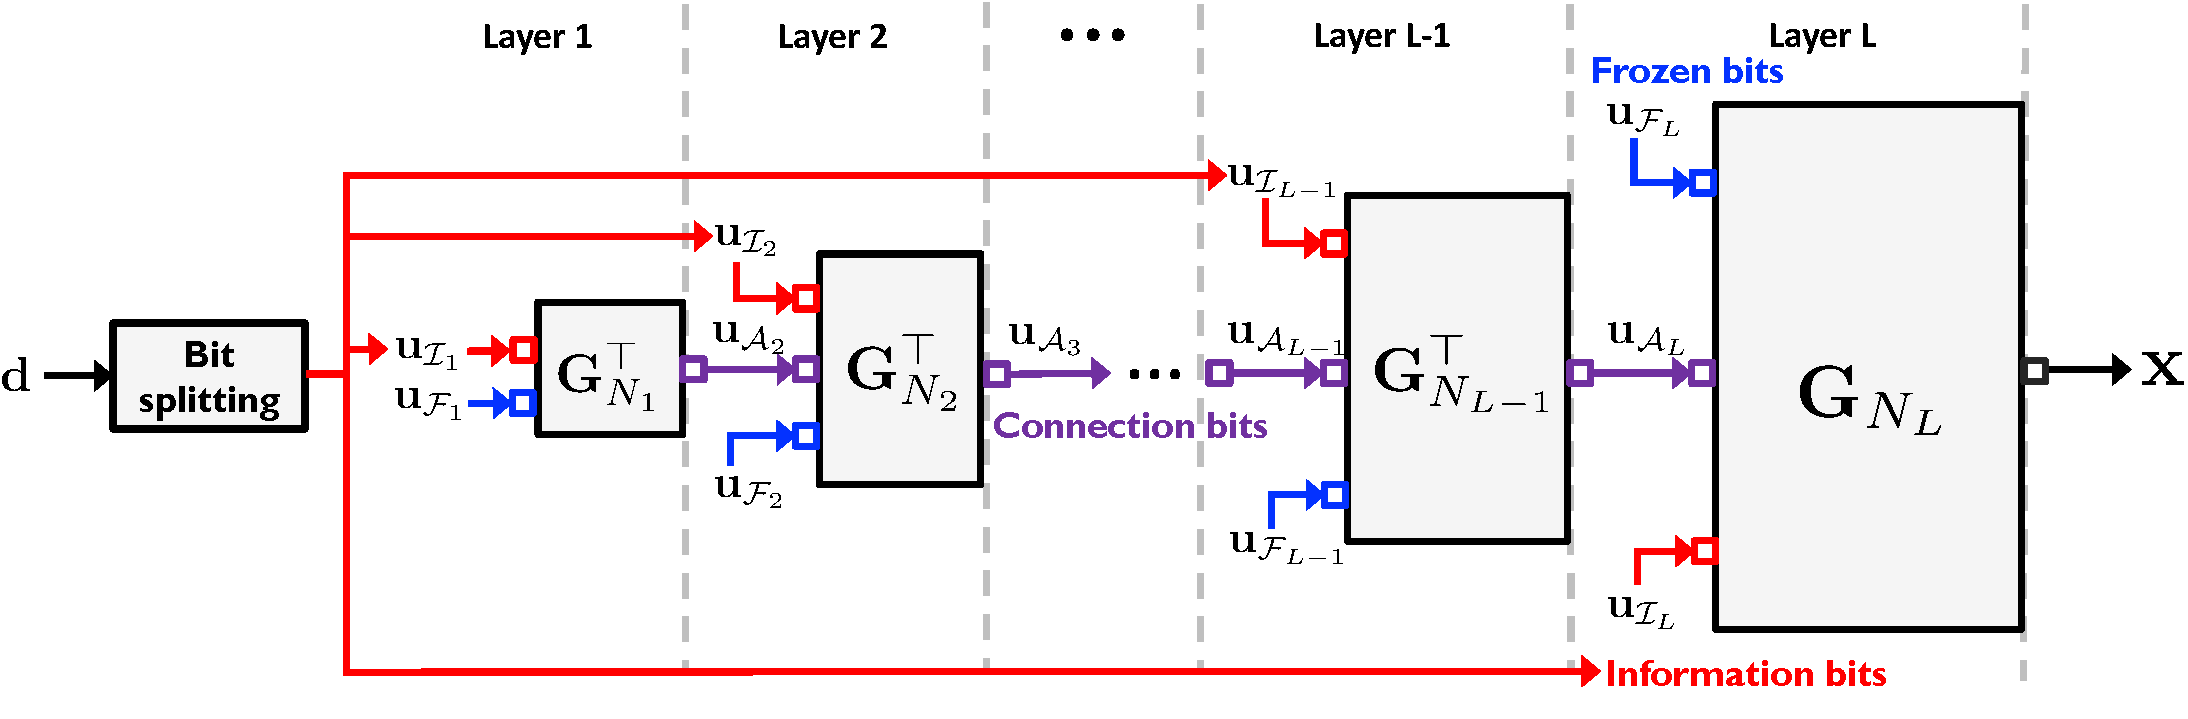
\includegraphics[width=1.7\columnwidth]{Encoder.pdf}
\caption{An illustration of the proposed deep polar encoder with $L$ layers.}
\label{fig:encoder}
\end{figure*}
 
 
A  $\left(N,K, \{\mathcal{I}_{\ell}\}_{\ell=1}^L, \{\mathcal{A}_{\ell}\}_{\ell=1}^L, \{{\bf T}_{\ell}\}_{\ell=1}^L\}\right)$ deep polar code is defined with the following parameters:
\begin{itemize}
	\item  i) $L$ transformation matrices ${\bf T}_{\ell}\in \mathbb{F}_2^{N_{\ell}\times N_{\ell}}$,
	\item ii) $L$ information sets $\{\mathcal{I}_1,\mathcal{I}_2,\ldots, \mathcal{I}_{L}\}$, and
	\item iii) $L$ connection sets $\{\mathcal{A}_1,\mathcal{A}_2,\ldots, \mathcal{A}_{L}\}$.
\end{itemize}
 For given these parameters, the deep polar encoder performs  information bit splitting and successive encoding.
 
  \vspace{0.2cm}
 {\bf Information bit splitting and mapping:} 
The information vector ${\bf d} \in \mathbb{F}_2^K$ carrying $K$ information bits is splitted into $L$ information sub-vectors ${\bf d}_{\ell}$, each with size of $K_{\ell}=|\mathcal{I}_{\ell}| (<N_{\ell})$ for ${\ell}\in [L]$ and $\sum_{\ell=1}^L K_{\ell}=K$. 

 Let ${\bf u}_{\ell}=[u_{\ell,1},u_{\ell,2},\ldots, u_{\ell, N_{\ell}}]\in \mathbb{F}_2^{N_{\ell}}$ be the input vector of layer $\ell$ with length $N_{\ell}$ for $\ell\in [L]$. The index set of the $\ell$th layer is partitioned into three non-overlapped sub-index sets as
 \begin{align}
 	[N_{\ell}] =\mathcal{I}_{\ell}\cup\mathcal{A}_{\ell}\cup \mathcal{F}_{\ell},
 \end{align}
 where $\mathcal{F}_{\ell}=[N_{\ell}]/\{\mathcal{I}_{\ell}\cup \mathcal{A}_{\ell}\}$ is the frozen bit set of layer $\ell$ and $\mathcal{I}_{\ell}\cap \mathcal{A}_{\ell}=\phi$.  The information vector of the $\ell$th layer, ${\bf d}_{\ell}\in \mathbb{F}_2^{K_{\ell}}$, is assigned to ${\bf u}_{\mathcal{I}_{\ell}}$. Meanwhile, the frozen bits are assigned to ${\bf u}_{\mathcal{F}_{\ell}}={\bf 0}$, where $\mathcal{F}_{\ell}=[N_{\ell}]/\{\mathcal{I}_{\ell}\cup \mathcal{A}_{\ell}\}$. 
 
 \vspace{0.2cm}
{\bf Successive encoding:} As depicted in Fig.~\ref{fig:encoder}, an $L$-layered deep polar code is constructed by $L$-stage successive encoding procedures. Let ${\bf T}_{\ell}\in \mathbb{F}_2^{N_{\ell}\times N_{\ell}}$ be the $\ell$th layered pre-transformation matrix where $N_{1}<N_{2}<\cdots <N_{L-1}<N_L$. Unlike the PAC or other PAC-like codes, our deep polar codes adopt the pre-transform matrix by multiplying the transpose of the polar transform matrix with length $N_{\ell}=2^{n_{\ell}}$ for $n_{\ell}\in \mathbb{Z}^{+}$ as
\begin{align}
	{\bf T}_{\ell}= {\bf G}_{N_{\ell}}^{\top}.
\end{align}
The primary feature is that the proposed pre-transformation matrix ${\bf T}_{\ell}= {\bf G}_{N_{\ell}}^{\top}$ not only facilitates easy calculations using fast polar transform but also has an upper triangular matrix structure. This upper triangular structure allows for improvement in the weight distribution of the code. 

%It is worth to note that we can use any pre-transform matrix ${\bf T}_{\ell}$ as long as it holds an upper triangular matrix structure with non-zero diagonal components.  


 In the first layer, the encoder generates the input vector of the first layer encoding, ${\bf u}_{1}=[  {\bf u}_{\mathcal{I}_{1}},~{\bf u}_{\mathcal{F}_{1}} ]$ where $\mathcal{A}_1=\phi$. The encoder output of the first layer is generated by ${\bf G}_{N_{1}}^{\top}$ as
\begin{align}
	{\bf v}_1 = {\bf u}_1{\bf G}_{N_{1}}^{\top}.
\end{align}
In the second layer,  the output vector of the first layer encoding is assigned to the input of the second layer to the connection index set $\mathcal{A}_2$, i.e., ${\bf u}_{\mathcal{A}_2}={\bf v}_1$. Since ${\bf u}_{\mathcal{I}_2}={\bf d}_2$ and ${\bf u}_{\mathcal{F}_2}={\bf 0}$, the input vector of the second layer encoding is 
\begin{align}
	{\bf u}_{2}=[  {\bf u}_{\mathcal{I}_{2}},~ {\bf u}_{\mathcal{A}_{2}},~{\bf u}_{\mathcal{F}_{2}} ].
\end{align} 
By multiplying ${\bf u}_{2}$ with ${\bf G}_{N_{2}}^{\top}$, the output vector of the second layer encoding is obtained as
\begin{align}
	{\bf v}_2 = {\bf u}_2 {\bf G}_{N_{2}}^{\top}.
\end{align}
Similar to the second layer encoding, the $\ell$th layer encoder for $2< \ell \leq L$ takes the input vector
\begin{align}
	{\bf u}_{\ell}=[  {\bf u}_{\mathcal{I}_{\ell}},~ {\bf u}_{\mathcal{A}_{\ell}},~{\bf u}_{\mathcal{F}_{\ell}} ],
\end{align} 
where ${\bf u}_{\mathcal{A}_{\ell}}={\bf u}_{\ell-1} {\bf G}_{N_{\ell-1}}^{\top}$, and generates the corresponding output vector by multiplying $ {\bf G}_{N_{\ell}}^{\top}$ or ${\bf G}_{N_L}$ as 
\begin{align}
{\bf v}_{\ell} &= 
\begin{cases}
	{\bf u}_{\ell}{\bf G}_{N_{\ell}}^{\top} & 2< \ell < L, \\
    {\bf u}_{L}{\bf G}_{N_{L}} & \ell = L. \\
\end{cases} \label{eq:encode}
\end{align}
For notational simplicity, we denote the output of the last layer encoder as the channel input ${\bf x}={\bf v}_L \in \mathbb{F}_2^{N_L}$.




%In the first layer, the encoder generates the input vector of the first layer ${\bf u}_{1}=[  {\bf u}_{\mathcal{I}_{\ell}},~{\bf u}_{\mathcal{F}_{1}} ]$ and constructs the corresponding output vector using the bit-reversed polar transform ${\bf G}_{N_{1}}^{\top}$ as
%\begin{align}
%	{\bf c}_1 = {\bf u}_1{\bf G}_{N_{1}}^{\top}.
%\end{align}
%From the second layer to the $L$th layer, the encoder generates the input vector 
%\begin{align}
%	{\bf u}_{\ell}=[  {\bf u}_{\mathcal{I}_{\ell}},~ {\bf u}_{\mathcal{A}_{\ell}},~{\bf u}_{\mathcal{F}_{\ell}} ]
%\end{align} 
%with ${\bf u}_{\mathcal{A}_{\ell}}={\bf c}_{\ell-1}$. Then, multiplying ${\bf u}_{\ell}$ to ${\bf G}_{N_{\ell}}^{\top}$, the encoder generates the output of the $\ell$th layer as \begin{align}
%	{\bf c}_{\ell} = {\bf u}_{\ell}{\bf G}_{N_{\ell}}^{\top}
%\end{align}
%for $\ell\in \{2,3,\ldots, L\}$ 

% our pre-transformation technique has potential to improve the coding performance as in [REF].  
   
 




%
%A deep polar code is constructed from $L$ successive polar encoding processes, each with different sizes of the polar transformation. Let  define the input and output vectors of the $\ell$th layer encoding as ${\bf u}_{\ell}=[u_{\ell,1},\ldots, u_{\ell,N_{\ell}}] \in \mathbb{F}_2^{N_{\ell}}$ and ${\bf c}_{\ell}=[c_{\ell,1},\ldots, c_{\ell,N_{\ell}}] \in \mathbb{F}_2^{N_{\ell}}$ for $\ell\in [L]$.  Unlike the conventional polar and PAC codes, a deep polar code needs three types of the index sets for the $\ell$th layer encoding. The $\ell$th layer encoder involves the three index sets:
%\begin{itemize}
%	\item 1) Information set $\mathcal{I}_{\ell}\subset [N_{\ell}]$ with $|\mathcal{I}_{\ell}|=K_{\ell}$ for $\ell\in [L]$; this set specifies the positions that carry the $K_{\ell}$ information bits in ${\bf u}_{\ell}$;
%	\item 2) Connection set $\mathcal{A}_{\ell}\subset [N_{\ell}]$ with $|\mathcal{A}_{\ell}|=N_{\ell-1}$ and $\mathcal{A}_{\ell}\cap \mathcal{I}_{\ell}=\phi$ for $\ell\in [L]$; this set indicates the indices of ${\bf u}_{\ell}$ that contains ${\bf c}_{\ell-1}$, i.e.,
%\begin{align}
%	\mathcal{A}_{\ell}=\{i\in [N_{\ell}]/\mathcal{I}_{\ell}: {u}_{\ell,i}={c}_{\ell-1,j}\},  
%\end{align}
% for $j\in [N_{\ell-1}]$. The connection set of the first layer is null, i.e., $\mathcal{A}_1=\phi$ because no prior layer is connected to the first layer. 
%  
% \item 3) Fronzen set $\mathcal{F}_{\ell}= [N_{\ell}]/\{\mathcal{I}_{\ell}\cup\mathcal{A}_{\ell}\}$ with $|\mathcal{F}_{\ell}|=(N_{\ell}-K_{\ell}-N_{\ell-1})^{+}$ for $\ell\in [L]$; The encoder assigns the zeros for the indices in ${\bf u}_{\ell}$, i.e., $u_{\ell,i}=0$ for $i\in \mathcal{F}_{\ell}$. 
% 
% 
%\end{itemize}
%


%Using these index sets, the encoder generates ${\bf u}_1, {\bf u}_2,\ldots, {\bf u}_{L}$ sequentially. 


% i) information $\mathcal{I}_{\ell}$, the connection $\mathcal{A}_{\ell}$, and frozen sets $\mathcal{F}_{\ell}$ for $\ell\in [L]$. 
%
%Let $\mathcal{I}_{\ell}\subset [N_{\ell}]$ with $|\mathcal{I}_{\ell}|=K_{\ell}$ be the information set that carries $K_{\ell}$ information bits in layer $\ell$. 
%In general, the encoder requires three index sets for the $\ell$th layer encoding, i) the information set $\mathcal{I}_{\ell}$, the connection set $\mathcal{A}_{\ell}$, and the frozen set $\mathcal{F}_{\ell}$ for $\ell\in \{2,3,\ldots, L\}$. 
%





%Multiplying ${\bf u}_{\ell}$ to ${\bf G}_{N_{\ell}}^{\top}$, the encoder generates the output of the $\ell$th layer encoding 
%\begin{align}
%	{\bf c}_{\ell} &= {\bf u}_2{\bf G}_{N_{2}}^{\top}\end{align} 
%for $\ell\in \{2,3,\ldots, L\}$.  As a result, 
%
%Specifically, for the first layer encoding, the encoder assigns $K_1$ information bits to the $K_1$ positions of the first layer input vector ${\bf u}_1$. The sub-vector carrying the information bits with $\mathcal{I}_{1}$ is denoted by ${\bf u}_{\mathcal{I}_{1}}$. In addition, the $N_1-K_1$ frozen bits are mapped into the remaining elements of ${\bf u}_1$, i.e., ${\bf u}_{\mathcal{F}_1}={\bf 0}$, where $\mathcal{F}_1\in [N_1]/\mathcal{I}_{1}$. Then, applying the bit-reversed polar transformation matrix ${\bf G}_{N_{1}}^{\top}$, the output of the first layer encoder is generated as
%\begin{align}
%	{\bf c}_1 = {\bf u}_1{\bf G}_{N_{1}}^{\top}.
%\end{align}
%
%For the second layer encoding, the encoder maps $K_2$ information bits to ${\bf u}_2$ using $\mathcal{I}_2$, i.e., ${\bf u}_{\mathcal{I}_2}$. Unlike the first layer encoding, the encoder maps the output of the first layer ${\bf c}_1$ with length $N_1$ to the positions of ${\bf u}_2$.  Let $\mathcal{A}_2=\{i\in \mathcal{N}_2/\mathcal{I}_2: {u}_{2,i}={c}_{2,j}\}$ for $j\in [N_1]$ be a set connecting the first layer output to the second layer input, i.e., ${\bf u}_{\mathcal{A}_2}={\bf c}_1$. Selecting the frozen set of the second layer as $\mathcal{F}_2=\mathcal{N}_2/\{\mathcal{I}_2\cup \mathcal{A}_2\}$, the output of the second layer encoder is given by
%\begin{align}
%	{\bf c}_2 &= {\bf u}_2{\bf G}_{N_{2}}^{\top}.
%\end{align} 




 
	 
\subsection{Rate-Profiling}
The selection of information and connection sets in all layers, $\mathcal{I}_{\ell}$ and $\mathcal{A}_{\ell}$, determines the error-correcting performance of deep polar codes. Unfortunately, finding the optimal set selection algorithm is very challenging. In this paper, we propose a flexible rate-profiling method that can support versatile code rates while guaranteeing an improved code weight distribution. The proposed rate-profiling method is to construct $\mathcal{I}_{\ell}$ and $\mathcal{A}_{\ell}$ for $\ell\in [L]$ individually across the layers. 



%The key idea of the proposed rate-profiling is to use the polar rate-profiling to design information set the last layer $\mathcal{I}_L$

%The proposed rate-profiling method is simple

 
%The proposed rate-profiling is to select the information and connection sets, $\mathcal{I}_{\ell}$ and $\mathcal{A}_{\ell}$, independently across layers. Nonetheless, when connecting adjacent layers, the encoder carefully matches the ordered-index connection set $\mathcal{A}_{\ell}$ with the output vector of the $\ell-1$ layer, ${\bf c}_{\ell-1}$.    


\vspace{0.1cm}
{\bf Selection of $\mathcal{I}_{\ell}$ and $\mathcal{A}_{\ell}$:}  We explain how to select information and connection sets for the $\ell$th layer for $\ell\in \{1,\ldots, L\}$.  To construct $\mathcal{I}_{\ell}$ and $\mathcal{A}_{\ell}$ independently over the layers, suppose the channel input ${\bf x}_{\ell} \in \{0,1\}^{N_{\ell}}$ is formed by the transpose of polar transform ${\bf x}_{\ell}={\bf u}_{\ell}{\bf G}_{N_{\ell}}^{\top}$ for $\ell\in \{1,2,\ldots, L-1\}$ and the forward polar transform ${\bf x}_{L}={\bf u}_{L}{\bf G}_{N_{L}}$ for the last layer.  Then,  the codeword generated by layer $\ell$ encoder, ${\bf x}_{\ell}$, is assumed to be transmitted over an B-DMC, $W:  \mathcal{X}\rightarrow \mathcal{Y}$, which produces the channel output ${\bf y}_{\ell}$ for $\ell\in [L]$.  The $i$th bit-channel when using layer $\ell$ encoder is defined as
\begin{align}
    W_{N_{\ell}}^{(i)}\left({\bf y}_{\ell}, {\bf u}_{\ell,1:i-1} | u_{\ell,i}\right) = \sum_{{\bf u}_{\ell, i+1:N} \in \mathbb{F}_2^{N_{\ell}-i}} \frac{1}{2^{N_{\ell}-i}} W^{N_{\ell}}\left({\bf y}_{\ell}  | {\bf x}_{
    \ell}\right),
\end{align}
where $i\in [N_{\ell}]$, ${\bf u}_{\ell, a:b}=[u_{\ell,a},u_{\ell, a+1},\ldots, u_{\ell,b}]$ for $a,b\in [N_{\ell}]$ and $a<b$.  Let $I\left(W_{N_{\ell}}^{(i)}\right)$ be the $i$th bit-channel capacity.  

To construct $\mathcal{I}_{\ell}$ and $\mathcal{A}_{\ell}$, we first define an index set $\mathcal{R}_{\ell}$ according to the RM rate-profiling by selecting $i\in [N_{\ell}]$ such that the weight of the rows ${\bf G}_{N_{\ell}}$ is equal to or larger than the pre-determined ${\sf d}_{\ell}^{\rm min}$, i.e., 
 \begin{align}
	\mathcal{R}_{\ell}=\{i\in [N_{\ell}]:  {\sf wt}\left({\bf g}_{N_{\ell},i} \right)\geq {\sf d}^{\rm min}_{\ell} \},
\end{align}
where ${\sf d}^{\rm min}_{\ell}$ is a target minimum distance for the $\ell$th layer encoding. Next, we define an ordered index set of $\mathcal{R}_{\ell}$ as
\begin{align}
    \mathcal{\bar R}_{\ell}=\left\{i_1,i_2,\ldots, i_{|\mathcal{R}_{\ell}|}\right\},
\end{align}
 where $i_1$ is the index of the most reliable synthetic channel, i.e., $ I\left(W_{N_{\ell}}^{(i_1)}\right) \geq I\left(W_{N_{\ell}}^{(i_2)}\right)\geq \cdots \geq I\left(W_{N_{\ell}}^{(i_{|\mathcal{R}_{\ell}|})}\right)$. This ordered set can be constructed using the ordered Bhattacharyya values, i.e., $Z\left(W_{N_{\ell}}^{(i_1)}\right)\leq Z\left(W_{N_{\ell}}^{(i_2)}\right),\ldots \leq Z\left(W_{N_{\ell}}^{(i_{|\mathcal{B}_{\ell}|})}\right)$ or the values obtained from the density evolution with Gaussian approximation technique in \cite{Tal-polar-construction, Trifnov-polar-construction}.  Using the ordered index set, the information set $\mathcal{I}_{\ell}$ is generated by selecting the bit-channel indices that are approximately polarized to the capacity of one for given code length $N_{\ell}$:
\begin{align}
	\mathcal{I}_{\ell}=\left\{i\in \mathcal{\bar R}_{\ell}: I\left(W_{N_{\ell}}^{(i)}\right) \geq 1-\delta_{\ell} \right\},
\end{align}
where $\delta_{\ell}>0$ is chosen arbitrary small and $|\mathcal{I}_{\ell}|=K_{\ell}$.



 
%In a finite block length $N_{L}$, the channel polarization is not sufficiently pronounced.  As a result, the number of the perfectly polarized bit-channels to the capacity is smaller than the target information bits $K$, i.e.,  

 Next, we construct the connection set $\mathcal{A}_{\ell}$ as a subset of $\mathcal{\bar R}_{\ell}/\mathcal{I}_{\ell}$. Let $j_1,j_2,\ldots, j_{N_{\ell-1}} \in \mathcal{R}_{\ell}/\mathcal{I}_{\ell}$ be the indices that provide the highest $N_{\ell-1}$ bit-channel capacities in $\mathcal{R}_{\ell}/\mathcal{I}_{\ell}$ such that  $ I\left(W_{N_{\ell}}^{(j_1)}\right) \geq I\left(W_{N_{\ell}}^{(j_2)}\right)\geq \cdots \geq I\left(W_{N_{\ell}}^{(j_{N_{\ell-1}})}\right)$. Then,
\begin{align}
	\mathcal{ A}_{\ell}=\left\{j_1,j_2,\ldots, j_{N_{\ell-1}}\right\}.
\end{align}
 The frozen set of layer $\ell$ is defined as the collection of indices that are excluded in both the information and connection sets as
\begin{align}
	\mathcal{F}_{\ell}=[N_{\ell}]/\{\mathcal{I}_{\ell}\cup \mathcal{A}_{\ell}\}.
\end{align}
This rate-profiling method is performed independently over the layers. 

% It is worth mentioning that the deep polar codewords generated by the proposed information and connection sets per layer ensure the minimum distance of ${\sf d}^{\rm min}_{\ell}$.


 \subsection{Remarks}
We provide some remarks on the encoding complexity, the superposition property, the minimum distance of the code, the concatenation with CRC codes, and the rate-compatibility.
  
 
 
% The proposed deep polar code can be considered a generalized version of the standard polar code. The standard polar code can be viewed as a deep polar code with a single layer that has a null connection set. Furthermore, our deep polar code serves as an alternative form of the pre-transformed polar code, which includes PAC codes.
 {\bf Encoding complexity:}  The proposed successive encoder composed of $L$ layers requires to take $L$ polar transformations, each with $N_{\ell}$ size. Since the computation of the polar transform with size $N_{\ell}$ needs the complexity of $\mathcal{O}(N_{\ell}\log_2 N_{\ell})$, the total encoding complexity boils down to
\begin{align}
	\mathcal{O}\left(\sum_{\ell=1}^LN_{\ell}\log_2 N_{\ell}\right).
\end{align}
It is worth mentioning that the encoding complexity can be comparable to that of the standard polar codes when $N_L$ is sufficiently larger than $N_{\ell}$ for $\ell\in [L-1]$. Choosing a small size of $N_{\ell}$ for $\ell\in [L-1]$ is a practical and effective strategy for reducing the encoding complexity.


\vspace{0.1cm}


{\bf Superposition codes :}  The deep polar code can be viewed with a lens through a superposition code of both the polar and the transformed polar codes as 
\begin{align}
 	{\bf x} = \underbrace{\sum_{j\in \mathcal{I}_{L}}u_{L,j} {\bf g}_{N_L, j} }_{{\bf x}_{\sf P}}+ \underbrace{\sum_{i\in \mathcal{A}_{L}}u_{L,i} {\bf g}_{N_L, i}}_{{\bf x}_{\sf TP}},
 \end{align}
where ${\bf x}_{\sf P}$ and  ${\bf x}_{\sf TP}$ represent polar and pre-transformed polar subcodewords, respectively. This superposition code interpretation provides a useful guideline for designing a low-complexity decoder while improving the weight distribution. Specifically, the pre-transformed subcodewords play a crucial role in improving the weight distribution of the deep polar code. The polar subcodewords facilitate to use a simple SC decoding because the information bits ${\bf u}_{\mathcal{I}_{L}}$ are sent through almost perfectly polarized bit-channels when the connection bits ${\bf u}_{\mathcal{A}_{L}}$ are treating as additional frozen bits. As a result, the deep polar codes offer a desirable balance between code performance and decoding complexity by strategically allocating information bit sizes between ${\bf u}_{\mathcal{I}_{L}}$ and ${\bf u}_{\mathcal{A}_{L}}$. For instance, when the blocklength goes to infinity, the encoder allocates all information bits to ${\bf u}_{\mathcal{I}_{L}}$ while $\mathcal{A}_{L}=\phi$; the deep polar codes boil down to a standard polar code.  

 
 

 {\vspace{0.1cm}}

 {\bf The minimum distance and weight distribution:} The minimum distance of the deep polar codes is larger or equal to the minimum distance of layer $L$, ${\sf d}_{L}^{\rm min}$.  By the construction, the encoder chooses the row vectors of ${\bf G}_{N_L}$ with the weight larger than ${\sf d}_{L}^{\rm min}$, namely, 
 \begin{align}
{\sf wt}\left( {\bf g}_{N_L, j}\right)	\geq {\sf d}_{L}^{\rm min}
 \end{align}
for $j\in \mathcal{I}_L \cup \mathcal{A}_L$. Since the pre-transform matrix of layer $L-1$ holds the upper triangular structure, the minimum distance of the pre-transformed subcodewords ${\bf x}_{\sf TP}=\sum_{i\in \mathcal{A}_{L}}u_{L,i} {\bf g}_{N_L, i}$ cannot be less than ${\sf d}_{L}^{\rm min}$.


% {\vspace{0.1cm}}
 
% {\bf Weight distribution improvement:} deep polar codes, like other pre-transformed polar codes, have an enhanced weight distribution compared to conventional polar codes. This is attributed to the generation of a sub-codeword ${\bf x}_{\sf TP}$ through partial pre-transforms with multiple layers.




%
% {\bf Flexible connection set construction:}
%To provide further flexibility in layer connections when the size of $\mathcal{A}_{\ell}$ is not equal to $2^{N_{\ell}}$, it is feasible to construct the pre-transform matrix of the $\ell$th layer as a sub-matrix of ${\bf G}_{N_{\ell}}^{\top}$ by selecting its columns. This construction enhances the adaptability of the layer connections in the system.






 {\vspace{0.1cm}}
 
 {\bf CRC-aided (CA) deep polar codes:} 
One possible extension of deep polar codes is to concatenate them with CRC codes. In this approach, the $K$-bit information vector ${\bf d}$ is precoded by using CRC generator polynomials, adding CRC bits. The length of the resulting information sequence becomes $K+K_{\rm CRC}$, where $K_{\rm CRC}$ represents the number of CRC bits. Alternatively, multiple CRC bits, each with short length, can be appended to the information bits of each layer, i.e., ${\bf u}_{\mathcal{I}_{\ell}}$ for $\ell\in [L]$ to improve the decoding performance. The effect of CRC code concatenation with the deep polar codes will be discussed in the simulation section. 
 
 
 {\vspace{0.1cm}}
 
 {\bf Rate-compatibility:} 
A design of rate-compatible codes suitable for hybrid automatic repeat request (HARQ) is an important feature for practical communication systems. Our deep polar code possesses a rate-compatible property, thanks to its multi-layered successive encoding structure. Suppose a transmitter sends a codeword ${\bf x}$ and a receiver fails to decode the message bits ${\bf d}$. Then, in the next round of the transmission, the transmitter sends only the output of $L-1$ layer, ${\bf u}_{\mathcal{A}_L}$, with blocklength of $N_{L-1}$ for enabling HARQ communications. The receiver attempts to decode the message by using both the noisy connection bits received in the second round and the received signal in the first round. This re-transmission and decoding protocol can be iteratively applied to the first layer, enhancing the decoding performance while reducing the code rates from $R=\frac{K}{N_L}$ to $R=\frac{K}{\sum_{\ell=1}^LN_{\ell}}$. Notwithstanding the flexible rate-compatibility, a delicate code optimization is required to 
attain a high HAQR performance by carefully choosing the blocklengths $N_{\ell}$ and information bits $K_{\ell}$ for each layer $\ell\in \{1,2,\ldots,L-1 \}$. Solving this optimization problem remains as a promising future topic.


% {\vspace{0.1cm}}
%
% {\bf Difference with the classical concatenated codes:} 
%
% The proposed deep polar codes can be viewed with a lens through a family of concatenated codes. Unlike the classical concatenation method, the output vector of the $\ell$th layer encoder is used as the partial input of the $\ell+1$th layer encoder. In addition, the classical concatenated codes are composed of inner and outer codes. Whereas, our construction utilizes multiple layered encoding structure, which can provide more flexibility in bit mapping.  
%  



%{\bf Connection between layers:} We explain how to connect the encoder output of $\ell-1$th layer, ${\bf v}_{\ell-1}\in \{0,1\}^{N_{\ell-1}}$ to the input of the $\ell$th layer, i.e., ${\bf u}_{\mathcal{A}_{\ell}}$. Let ${\bf P}_{\ell}\in \mathbb{F}_2^{N_{\ell}\times N_{\ell}}$ be a permutation matrix. Then, using this permutation matrix, we define the connection between ${\bf v}_{\ell-1}$ and ${\bf u}_{\mathcal{A}_{\ell}}=[u_{\ell_1}, u_{\ell_2},\ldots u_{\ell_{N_{\ell}}}]$ as
%\begin{align}
%[u_{\ell_1}, u_{\ell_2},\ldots u_{\ell_{N_{\ell}}}]=[v_{\ell-1,1}, v_{\ell-1,2},\ldots, v_{\ell-1,N_{\ell}}]{\bf P}_{\ell}.
%\end{align}


 

\section{Examples }
In this section, we provide some examples of the design of deep polar codes in a short blocklength regime to better understand the proposed encoding method.  Throughout the examples, we shall focus on a short packet transmission scenario with a length of $32$ over a BEC with an erasure probability of 0.5, i.e., $I(W)=0.5$ at two different rates $R\in \{\frac{11}{32},\frac{15}{32}\}$. 


\subsection{Channel Polarization and Row Weights of ${\bf G}_{32}$}

For a deep polar code construction, it is important to understand the polarized bit-channel capacities and the row weight of ${\bf G}_{32}$. As shown in Fig. \ref{fig:rateprofiling}, the red circles indicate the bit-channel capacities for the BEC with $I(W)=0.5$, i.e., $I\left(W_{32}^{(i)}\right)$ for $i\in [32]$. The blue cross indicates the normalized weight of ${\bf G}_{32}$ according to index $i\in [32]$, i.e., $\frac{{\sf wt}({\bf g}_{32,i})}{32}$. The ordered index sets are mismatched according to bit-channel capacities and the normalized weights. For instance, $I\left(W_{32}^{(25)}\right)> I\left(W_{32}^{(12)}\right)$ but $\frac{{\sf wt}({\bf g}_{32,25})}{32} < \frac{{\sf wt}({\bf g}_{32,12})}{32}$.  When including the bit-index 25 in the information set to facilitate SC decoding, the minimum distance of the codewords is necessarily reduced. It becomes crucial to carefully select the bit-indices to improve the coding performance, considering both their weights and the bit-channel capacities. 

%Throughout the following examples, we explain how to effectively choose the information and connection sets to construct two-layered deep polar codes at two different rates.


\begin{figure}[t]
\centering
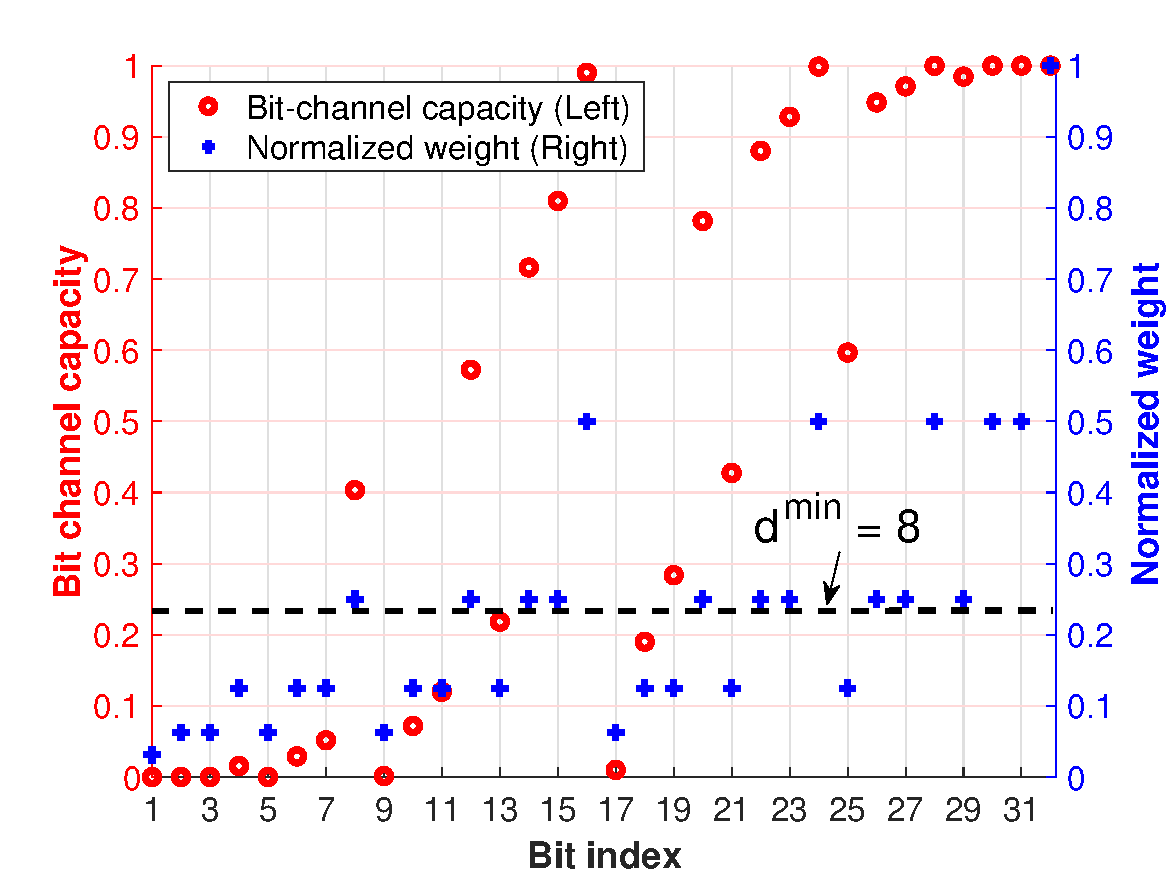
\includegraphics[width=1\columnwidth]{RateProfiling.pdf}
\caption{Polarized bit-channel capacity (left) and normalized weight (right) for the BEC with $I(W)=0.5$.}
\label{fig:rateprofiling}
\end{figure}

 
%We explain the rate-profiling method for the deep polar code construction through the following examples.  

\subsection{Example 1}
 

This example explains how to construct a two-layered deep polar code with a code rate of $R=\frac{11}{32}$. The encoding process involves utilizing two transformation matrices: ${\bf G}_{8}^{\top}$ for layer 1 and ${\bf G}_{32}$ for layer 2.  Assuming that a target minimum distance of the second layer is ${\sf d}^{\rm min}_{2}=8$, we select the indices of rows in the matrix ${\bf G}_{32}$ whose weights are greater than or equal to ${\sf d}^{\rm min}_{2}=8$, i.e.,
 \begin{align}
	\mathcal{R}_{2}=\{8,12,14,15,16,20,22,23,24,26,27,28,29,30,31,32\}.\nonumber
\end{align}
Then, from Fig. \ref{fig:rateprofiling}, the information set for the second layer, a subset of $\mathcal{R}_{2}$, is chosen as
\begin{align}
	\mathcal{I}_2&=\left\{i\in \mathcal{R}_2: I\left(W_{32}^{(i)}\right) \geq 0.98 \right\}\nonumber\\
	& =\{32,31,30,28,24,16,29\},\nonumber
\end{align}
where $|\mathcal{I}_2|=K_2=7$.  Considering that $N_1=8$, we identify the eight bit-channel indices that yield the highest capacity in $\mathcal{R}_2/\mathcal{I}_2$ to form the connection set for the second layer as
  \begin{align}
	\mathcal{A}_2 =\{ 27,26,23,22,15,20,14,12\}.\nonumber
\end{align}
It is worth mentioning that the bit-channel index of $25$ was excluded in the connection set although its capacity is larger than that of the index of $12$, i.e.,  $I\left(W_{32}^{(25)}\right) \geq I\left(W_{32}^{(12)}\right)$. This is because ${\sf wt}\left({\bf g}_{32,25} \right)=4<{\sf wt}\left({\bf g}_{32,12} \right)=8$. The frozen set of the second layer becomes
\begin{align}
	\mathcal{F}_2=\{1,2,\ldots, 32\}/\{\mathcal{I}_2\cup\mathcal{A}_2\}.\nonumber
\end{align}
In the first layer, we identify the four indices that result in the highest bit-channel capacity using the polar transform matrix ${\bf G}_8^{\top}$, while ensuring that the minimum distance ${\sf d}^{\rm min}_1$ is greater than or equal to 4. The corresponding information and frozen sets are chosen as $\mathcal{I}_1=\{1,2,3,5\}$ and $\mathcal{F}_1=\{8,7,6,4\}$, respectively. The output vector of the first layer, denoted as ${\bf v}_1={\bf u}_{1}{\bf G}_8^{\top}$, is then connected to the input of connection set ${\bf u}_{\mathcal{A}_2}={\bf v}_1$.


\begin{table}
\centering
\caption{Comparison of the weight distributions }\label{table:WD}
\begin{tabular}{c|ccc|cccccc}
\toprule
{} & {} & $[32,11]$ & {} & {} & $[32,15]$  & {} \\ 
\cmidrule(lr){1-1}\cmidrule(lr){2-4}\cmidrule(lr){5-7}
{Weight} & Polar & RM-type & Proposed & Polar & RM-type & Proposed \\ 
\midrule
$0$  &  $1$        &  $1$     &  $1$          & $1$           &  $1$            &  $1$\\
$4$  &  $0$        &  $0$     &  $0$          & $8$           &  $0$            &  $0$\\
$8$  & $76$       &  $40$   &  $20$        & $444$       &  $364$        &  $300$\\
$12$ & $192$     &  $336$  &  $416$      & $6328$     &  $6720$      &  $6976$\\
$16$ &  $1510$  &  $1294$ &  $1174$    & $19206$   &  $18598$    &  $18214$\\ 
$20$ & $192$     &  $336$  &  $416$       & $6328$    &  $6720$      &  $6976$\\  
$24$ & $76$       &  $40$    &  $20$        & $444$       &  $364$       &  $300$\\
$28$ & $0$         &  $0$     &  $0$           & $8$          &  $0$           &  $0$\\
$32$ & $1$         &  $1$     &  $1$           & $1$          &  $1$           &  $1$\\
\bottomrule
\end{tabular}
\end{table}
 
 
\subsection{Example 2}
We present an additional example to construct an $\left(32,15, \{\mathcal{I}_1, \mathcal{I}_2\}, \{\phi, \mathcal{A}_2\}, \{{\bf G}_{4}^{\top}, {\bf G}_{32}\}\right)$ deep polar code. Applying the same approach as in Example 1, we first select the indices corresponding to the row vectors of ${\bf G}_{32}$ with a weight greater than 8 in an identical manner as  \begin{align}
 	\mathcal{R}_{2}=\{8,12,14,15,16,20,22,23,24,26,27,28,29,30,31,32\}.\nonumber
 \end{align}
We adopt the deep polar rate-profiling method by selecting the information and connection sets as
\begin{align}
	\mathcal{I}_2=\{15,16,22,23,24,26,27,28,29,30,31,32\}\nonumber
\end{align}
with $K_2=|\mathcal{I}_2|=12$
and
\begin{align}
	\mathcal{A}_2=\{8,12,14,20\}.\nonumber
\end{align}
Then, we choose the information set for the first layer as
\begin{align}
	\mathcal{I}_1=\{1,2,3\}\nonumber
\end{align}
with $K_1=|\mathcal{I}_{1}|  =3$. 


%\vspace{0.2cm}
%{\bf Comparison:} 

\subsection{Comparisons with RM-type and Polar Codes}

We compare our deep polar codes in Examples 1 and 2 with existing RM and polar codes. We generate the polar codes for fair comparison by selecting the top $K\in \{11,15\}$ bit-channel indices that provide the highest capacities. For the RM code construction with information bit size $K\in \{11,15\}$,  we consider a subcodeword set of a $[32,16]$ RM code. Since the information set of the $[32,16]$ RM code is 
\begin{align}
	\mathcal{I}_{\sf RM}^{16} =\{i: {\sf wt}({\bf g}_{32,i})\geq 8\},
\end{align}
we choose the information set for $K=15$ as a subset of $ \mathcal{I}_{\sf RM}^{16}$, i.e., $\mathcal{I}_{\sf RM}^{15}\subseteq \mathcal{I}_{\sf RM}^{16}$. In particular, to optimize the code performance, we evaluate the weight distributions of 16 possible sub-codebooks of the $[32,16]$-RM code and select the best one with the smallest number of the codewords with the minimum weights. 
 

\vspace{0.1cm}
{\bf Weight distribution:}
As shown in Table \ref{table:WD}, the proposed deep polar codes provide superior weight distributions than those of the RM and polar codes in both code rates. Specifically, deep polar codes have fewer codewords having the minimum weight than the RM codes while keeping the identical minimum distance of $8$ in both code rates. In addition, the deep polar code with a rate of $R=\frac{15}{32}$ can improve both the minimum distance and the number of codewords having the smallest weights. 


%\vspace{0.1cm}
{\bf BLER performance:}
To demonstrate the effect of the weight distribution improvement in the code design, we plot BLERs for the three codes under ML decoding as increasing the erasure probabilities of the BEC. As illustrated in Fig. \ref{fig:BLER_BEC}, the proposed deep polar provides noticeable BLER improvement compared to the RM and polar codes when $K=11$. This BLER gain stems from the considerable reduction of the codewords with the minimum weight. When $K=15$, the minimum distance of deep polar and RM codes is larger than the polar code, which leads to improved BELR performance. Although the deep polar and RM codes have identical minimum distances, the deep polar code slightly outperforms the RM code by reducing the codewords with the minimum weight, as shown in Table \ref{table:WD}. One remarkable result is that the deep polar codes can achieve better BLER performances than the dependence-testing (DT) bound, one of the strongest achievability bounds for the BEC in the finite blocklength regime. 

%The results  indicate that the deep polar code has  a potential to achieve the capacity of the BEC with a small gap in short blocklength regimes with various code rates. 
 
 
  \begin{figure}[t]
\centering
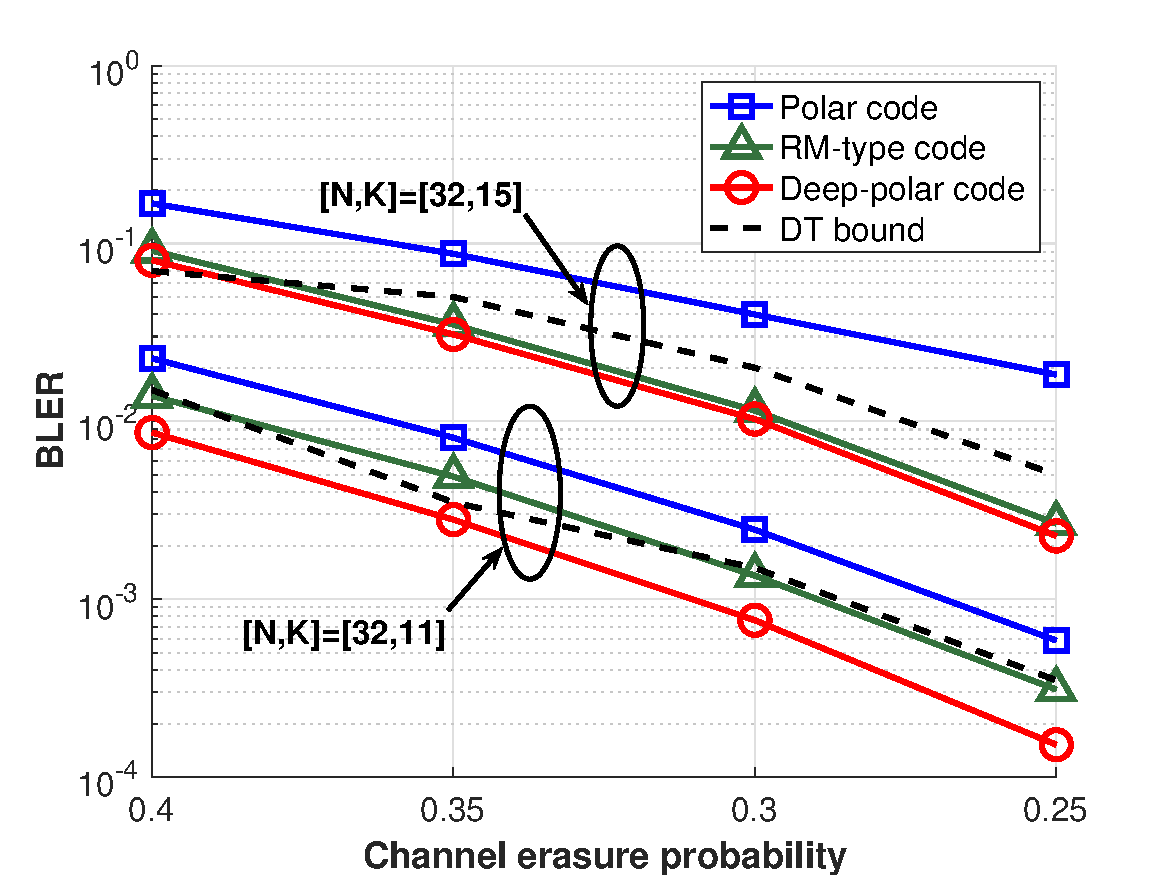
\includegraphics[width=0.9\columnwidth]{BLER_BEC.pdf}
\caption{BLER performance comparison for the BEC channel with $N=32$ and $K\in \{11,15\}$.}
\label{fig:BLER_BEC} \vspace{-0.5cm}
\end{figure}
\vspace{-0.1cm}



\vspace{0.1cm}

{\bf Pre-transform using a sub-upper triangular matrix:} In contrast to conventional pre-transformed polar codes that utilize an upper triangular matrix for pre-transformation, our resulting pre-transformation matrix across multiple layers can be seen as a sub-matrix of an upper triangular matrix. For instance, we express our two-layered encoding structure with a unified pre-transform matrix ${\bf T}\in \mathbb{F}_2^{32\times 32}$ as follows:
\begin{align}
	[{\bf u}_{\mathcal{F}_2}, {\bf u}_{1}, {\bf u}_{\mathcal{I}_2}]\underbrace{\begin{bmatrix}
{\bf 0}_{17} & {\bf 0}_{17} & {\bf 0}_{17} \\
{\bf 0}_8 &  {\bf G}_8^{\top}& {\bf 0}_8  \\
{\bf 0}_{7} & {\bf 0}_{7} & {\bf I}_{7}   
\end{bmatrix}}_{{\bf T}}{\bf G}_{32}={\bf x}.
\end{align}
It is evident that the resulting pre-transformed matrix ${\bf T}$ does not exhibit an upper diagonal structure; instead, a sub-matrix of ${\bf T}$ takes the form of an upper triangular matrix. This condition is less strict than the PAC and the existing pre-transformed polar codes, where the entire ${\bf T}$ matrix must be  Toeplitz or upper triangular.



 
\section{deep polar Decoders}
In this section, we present two decoding algorithms for deep polar codes. The first decoding method is SCL with backpropagation parity check (SCL-BPC), which provides flexibility in balancing complexity and performance through list size control. Motivated by the superposition code interpretation, the second algorithm is the parallel-SCL, which aims to reduce the decoding latency at the cost of increased hardware complexity. 

%These algorithms aim to reduce the decoding complexity or latency while improving the decoding performance of deep polar codes.


\subsection{SCL-BPC Decoder}


 The central concept behind SCL-BPC is to efficiently prune decoding paths that fail to satisfy the successive parity check equations within the deep polar encoder during the SCL decoding process.  As a stepping stone toward understanding the overall SCL-BPC decoder, it is instructive to explain the BPC mechanism used in decoding, which is the key ingredient of the proposed decoder. The key concept behind the BPC mechanism is to leverage the reverse process of the deep polar encoder. From \eqref{eq:encode}, the deep polar encoder generates the connection bits of layer $\ell\in [L]$, ${\bf u}_{\mathcal{A}_{\ell}}$, using the input of encoder at layer $\ell-1$ and ${\bf G}_{N_{\ell-1}}^{\top}$ as 
\begin{align}
	{\bf u}_{\mathcal{A}_{\ell}}=[  {\bf u}_{\mathcal{I}_{\ell-1}},~ {\bf u}_{\mathcal{A}_{\ell-1}},~{\bf u}_{\mathcal{F}_{\ell-1}} ] {\bf G}_{N_{\ell-1}}^{\top}.
\end{align} 
 From this successive encoder structure, we know that if ${\bf u}_{\mathcal{A}_{\ell}}$ is successfully decoded, the reverse encoding using ${\bf T}_{\ell-1}^{-1}={\bf G}_{N_{\ell-1}}^{\top}$ ensures to produce the frozen bits of the previous layer:
 \begin{align}
 	{\bf u}_{\mathcal{F}_{\ell-1}} =	\left({\bf u}_{\mathcal{A}_{\ell}}{\bf G}_{N_{\ell-1}}^{\top} \right)_{{\mathcal{F}_{\ell-1}}},
 \end{align}
 for $\ell\in \{2,3,\ldots, L\}$. Precisely estimating ${\bf \hat u}_{\mathcal{A}_{L}}$ is crucial for effective decoding using the BPC mechanism. However, accurately estimating the connection bits in layer $L$ presents a significant challenge due to their transmission over less reliable bit-channels than the information bits during SCL decoding. Consequently, incorrect estimation of ${\bf \hat u}_{\mathcal{A}_{L}}$ can lead to a degradation in the performance of SCL decoding, mainly when the list size is insufficiently large.




\begin{figure*}[t]
\centering
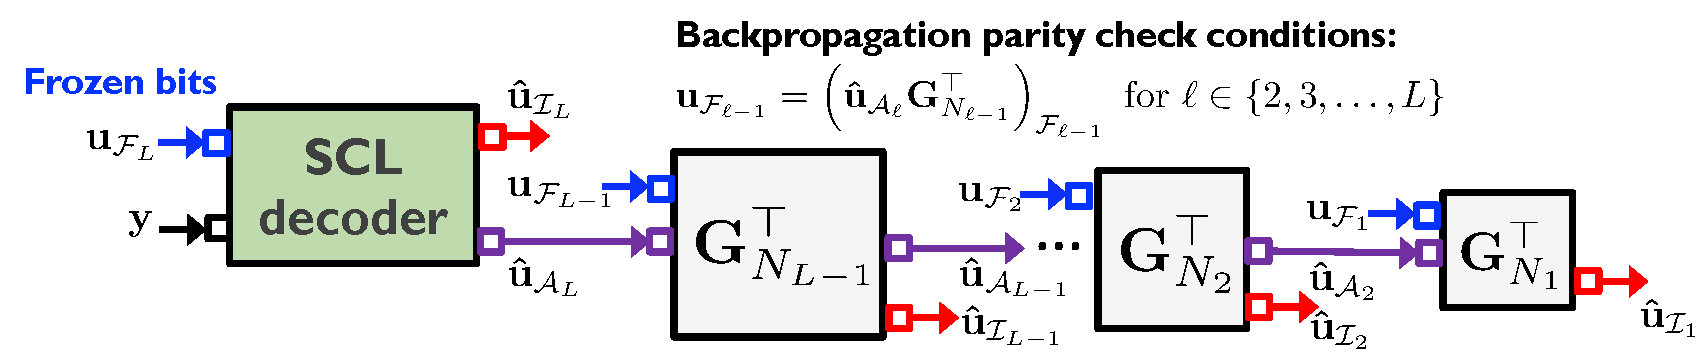
\includegraphics[width=1.6\columnwidth]{Decoder1.pdf}
\caption{An illustration of the SCL decoder using the backpropagation parity check principle.}
\label{fig:decoder}
\end{figure*}


\begin{algorithm}
\caption{ SCL-BPC Decoder}\label{alg:deep polar-SCL}
\KwData{List size $S$, channel output ${\bf y}$, transform matrices ${\bf T}_{\ell}$, information sets $\mathcal{I}_{\ell}$, connection sets $\mathcal{A}_{\ell}$, frozen sets $\mathcal{F}_{\ell}, ~ \forall \ell\in [L]$, and frozen bits ${\bf u}_{\mathcal{F}_L}$.}
% \KwResult{Estimated bits ${\bf \hat u}_{\mathcal{I}_{L}}, {\bf \hat u}_{\mathcal{A}_{L}}$}
\KwResult{Estimated information bits ${\bf \hat u}_{\mathcal{I}_{\ell}}[s^\star], ~ \forall \ell \in [L]$\;}
\vspace{0.2cm}
\emph{*** Initialization ***}\;
$\mathcal{P}_{\sf alive} \gets \{1\}$;
$\mathcal{P}_{\sf pool} \gets [2S]/\mathcal{L}_{\sf alive}$\; 
${\sf PM}[s] \gets 0, ~\forall s\in [S]$\;
\vspace{0.2cm}
\emph{*** Decoding ***}\;
\For(){$i=1,2,\ldots, N_L$}{
    \For(\tcp*[h]{path cloning}){$s\in \mathcal{P}_{\sf alive}$} {
        $\eta_i \gets \log \frac{ p\left({\bf y}, {\bf \hat u}_{L,1:i-1}[s] \vert u_{L,i} = 0\right) } { p\left({\bf y}, {\bf \hat u}_{L,1:i-1}[s] \vert u_{L,i} = 1\right) }$\;
        \eIf(\tcp*[h]{frozen bits}){$i\in \mathcal{F}_{L}$}{
            ${\hat u}_{L,i}[s] \gets u_{L,i}$\;
            ${\sf PM}[s] \gets {\sf PM}[s] + \log\left(1 + e^{-(1-2{\hat u}_{L,i}[s])\eta_i}\right)$\;}
            (\tcp*[h]{information bits}){
            Copy the path $s$ into a new path $s'\in \mathcal{P}_{\sf pool}$\;
            $\mathcal{P}_{\sf alive}\gets \mathcal{P}_{\sf alive} \cup \{s'\}$;
            $\mathcal{P}_{\sf pool} \gets \mathcal{P}_{\sf pool} / \{s'\}$\;
            ${\hat u}_{L,i}[s] \gets 0$; ${\hat u}_{L,i}[s'] \gets 1$\; 
            ${\sf PM}[s] \gets {\sf PM}[s] + \log\left(1 + e^{-(1-2{\hat u}_{L,i}[s])\eta_i}\right)$\;
            ${\sf PM}[s'] \gets {\sf PM}[s'] + \log\left(1 + e^{-(1-2{\hat u}_{L,i}[s'])\eta_i}\right)$\;          
        }
    }
    
    \If(\tcp*[h]{parity check}) {$i \in \mathcal{A}_{L}$}{
        \For {$s\in\mathcal{P}_{\sf alive}$} {
            Apply inverse transform according to \eqref{eqn:partial-inverse}\;
            ${\bf \hat u}_{\mathcal{F}_{\ell}, 1:k_{\ell}} \gets $ currently available frozen bits of layer $\ell\in[L]$\;
            \If {${\bf \hat u}_{\mathcal{F}_{\ell}, 1:k_{\ell}} \neq {\bf 0}$ for some $\ell$} {
                Kill the path $s$ \;
                $\mathcal{P}_{\sf alive}\gets \mathcal{P}_{\sf alive} /\{s\}$; $\mathcal{P}_{\sf pool} \gets \mathcal{P}_{\sf pool} \cup \{ s \}$ \;
            }
        }
    }    
    
    \If(\tcp*[h]{list pruning}) {$|\mathcal{P}_{\sf alive}| > S$} {
        $\tau_{\sf threshold} \gets$ the $S$th smallest ${\sf PM}[s]$ for $s\in\mathcal{P}_{\sf alive}$\;
        \For{${s}\in\mathcal{P}_{\sf alive}$}{
            \If {${\sf PM}[s] > \tau_{\sf threshold}$} {
                Kill the path $s$\;
                $\mathcal{P}_{\sf alive}\gets \mathcal{P}_{\sf alive} /\{s\}$; $\mathcal{P}_{\sf pool} \gets \mathcal{P}_{\sf pool} \cup \{ s \}$ \;
            }
        }
    }
}
Find $s^{\star}\gets \arg \min_{s\in \mathcal{P}_{\sf alive}} {\sf PM}[s]$\;
\vspace{0.2cm}
\emph{*** Information bits extraction ***}\;
\For{$\ell = L, \ldots, 2$}{
    ${\bf \hat u}_{\mathcal{I}_{\ell-1}}[s^\star] \gets \left( {\bf \hat u}_{\mathcal{A}_{\ell}}[s^\star] {\bf G}_{N_{\ell-1}}^{\top} \right)_{\mathcal{I}_{\ell-1}}$\;
    ${\bf \hat u}_{\mathcal{A}_{\ell-1}}[s^\star] \gets \left( {\bf \hat u}_{\mathcal{A}_{\ell}}[s^\star] {\bf G}_{N_{\ell-1}}^{\top} \right)_{\mathcal{A}_{\ell-1}}$\;
}
% Return ${\bf \hat u}_{\mathcal{I}_L}[s^{\star}]$ and ${\bf \hat u}_{\mathcal{A}_L}[s^{\star}]$\;
Return ${\bf \hat u}_{\mathcal{I}_{\ell}}[s^\star], ~ \forall \ell \in [L]$\;
\end{algorithm}

 
We propose an efficient SCL-BPC decoder by leveraging a bit-wise BPC mechanism to improve the decoding performance. The major idea is to verify the backpropagation syndrome check condition at the bit level within each layer, specifically for the elements denoted as $u_{L,i}$, where $i$ belongs to the set $\mathcal{A}_L$. To simplify our notation, we define ${\bf G}_{N_{\ell}, 1:k}^{\top} \in \mathbb{F}_2^{k\times k}$ as the upper-left submatrix of ${\bf G}_{N_{\ell}}^{\top}$. It is important to note that our pre-transform technique using the polar transform matrix possesses a unique property: its inverse is equal to itself. As a result, the inverse pre-transformation matrix is simply calculated itself as 
\begin{align}
    \left({\bf G}_{N_{\ell}, 1:k}^{\top}\right)^{-1} = {\bf G}_{N_{\ell}, 1:k}^{\top}, ~\forall \ell\in[L-1], \forall k\in[K].
\end{align}
If we denote the connection bits of layer $\ell$ as ${\bf \hat u}_{\mathcal{A}_{\ell}} = [{\hat u}_{\ell, i_{1}}, {\hat u}_{\ell, i_{2}}, \ldots, {\hat u}_{\ell, i_{N_{\ell-1}}}]$ such that $i_1 < i_2 < \cdots < i_{N_{\ell-1}}$, we express 
\begin{align}
    {\bf \hat u}_{\ell-1, 1:k} = {\bf \hat u}_{\mathcal{A}_{\ell}, 1:k} {\bf G}_{N_{\ell-1}, 1:k}^{\top}, \label{eqn:partial-inverse}
\end{align}
where ${\bf \hat u}_{\ell-1, 1:k}$ is a subsequence that comprises the first $k$ elements of ${\bf \hat u}_{\ell-1}$. Next, we extract two portions from the estimated bits ${\bf \hat u}_{\ell-1}$ of layer $\ell-1$: one portion is used for parity checking, and the other portion consists of connection bits that are recursively applied using  \eqref{eqn:partial-inverse}. Finally, we gather the estimated frozen bits from each layer $\ell \in [L]$ and verify their syndromes as depicted in Fig.~\ref{fig:decoder}.


Leveraging this bit-wise BPC mechanism, the proposed SCL decoder employs a level-by-level search strategy on a binary tree. At each bit $u_{L,i}$, where $i\in \mathcal{A}_L\cup \mathcal{I}_L$, the decoder extends the list of candidate paths by exploring both paths of the binary tree and appending either $u_{L,i}=0$ or $u_{L,i}=1$ to each candidate path. Consequently, the number of paths is doubled but limited to a predetermined maximum value $S$. In contrast to the standard SCL decoder, it is included in the list whenever a new path satisfies the BPC and ranks among the $S$ most reliable paths. Conversely, it is discarded if a new path fails the BPC or exhibits lower reliability than the existing $S$ paths in the list. This iterative process continues until $i\in [N_L]$. Ultimately, the decoder selects the path with the highest reliability metric as the output. When $S=1$, our decoder simplifies to the SC decoder utilizing the backpropagation parity check. The deep polar SCL decoding procedure is summarized in Algorithm~\ref{alg:deep polar-SCL}.
  
    The proposed decoder introduces an extra decoding complexity due to the BPC operation compared to the standard SCL decoding complexity with a list size of $S$, which is $\mathcal{O}(SN_L\log N_L)$. For each layer $\ell\in \{1,2,\ldots, N_{L-1}\}$, the parity check can be performed with a complexity of $\mathcal{O}(N_{\ell}\log N_{\ell})$. Consequently, the overall complexity is the sum of the complexity required for SCL decoding and computing the inverse of the pre-transforms, i.e.,
\begin{align}
	\mathcal{O}(SN_L\log N_L)+ \mathcal{O}\left(\sum_{\ell=1}^{L-1}N_{\ell}\log N_{\ell}\right).
\end{align} 
It is worth noting that the additional complexity introduced by the inverse of the pre-transform can be ignored when $N_L$ is significantly larger than $N_{\ell}$ for $\ell\in[L-1]$.




  \subsection{A Low-Latency Decoder }
  
   \begin{figure*}[t]
 \centering
 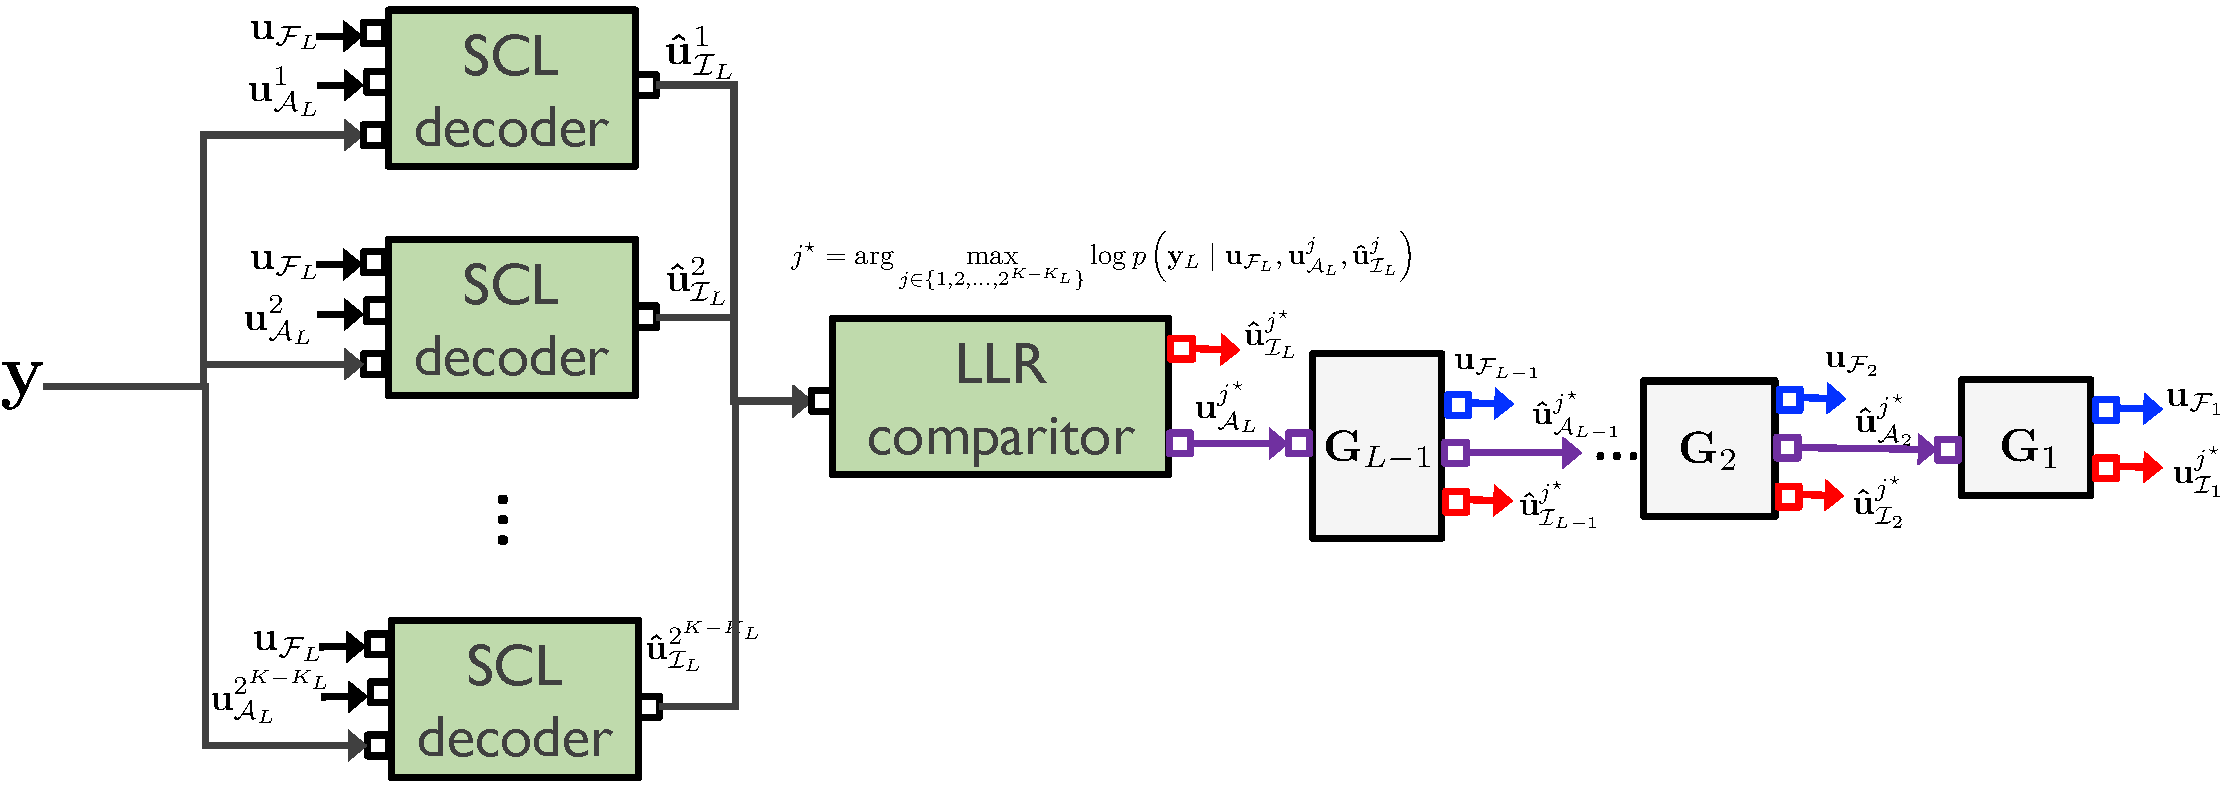
\includegraphics[width=1.7\columnwidth]{Decoder2.pdf}
 \caption{The proposed backpropagation decoding method using parallel-SCL decoders.}
 \label{fig:decoder-parallel}
 \end{figure*}
  
  
  
We also present a method for achieving low-latency decoding of deep polar codes. Our approach involves leveraging standard SCL decoders in parallel to estimate the information vector ${\bf u}_{\mathcal{I}_{L}}$, assuming the connection bits in layer $L$, ${\bf u}_{\mathcal{A}_{L}}$, as an additional frozen set alongside with frozen bits ${\bf u}_{\mathcal{F}_L}$. There are $2^{K-K_L}$ potential connection bit patterns for ${\bf u}_{\mathcal{A}_{L}}$. Let ${\bf u}_{\mathcal{A}_{L}}^j\in \mathbb{F}_2^{N_{L-1}}$ represent the $j$th connection bit pattern, where $j\in \left\{1,2,\ldots, 2^{K-K_L}\right\}$. Given the $j$th connection bit pattern ${\bf u}_{\mathcal{A}_{L}}^j$ and the frozen bits of the last layer ${\bf u}_{\mathcal{F}_{L}}={\bf 0}$, the SCL decoder identifies the most reliable information vector from a list of size $S$. Denoting the result of SCL decoding for the $j$th possible connection bit pattern and frozen bits as ${\bf \hat u}_{\mathcal{I}_{L}}^{j}$, the decoder selects the most reliable estimate ${\bf \hat u}_{\mathcal{I}_{L}}^{j^{\star}}$ for the information vector from the set $\{1,2,\ldots, 2^{K-K_L}\}$ as 
\begin{align}
 j^{\star}=\argmax_{j\in \{1,2,\ldots, 2^{K-K_L}\} }  \log p\left({\bf y}_L \mid {\bf u}_{\mathcal{F}_{L}}, {\bf u}_{\mathcal{A}_{L}}^j, {\bf \hat u}_{\mathcal{I}_{L}}^j\right).
\end{align}
The parallel-SCL decoding method diminishes the decoding latency by harnessing the power of parallel processing. However, the hardware complexity of this method increases exponentially with the number of information bits encoded in $\ell$ layers, where $\ell\in \{1,2,\ldots, L-1\}$ and $K-K_L$. Consequently, practical usage of this method is limited to scenarios where the number of $K-K_L$ is small enough. In addition, the overall computational complexity of the parallel-SCL decoding becomes 
\begin{align}
	\mathcal{O}\left(2^{K-K_L}SN_L\log N_L\right).
\end{align} 
The list size $S$ of this parallel-SCL decoding can be chosen very small because the information bits are sent through the bit-channels with the highest capacities under the premise that the actual connection bits are utilized as the frozen bits. Therefore, the implementation needs to carefully optimize the list size and the number of parallel-SCL decoders so that $2^{K-K_L}S$ is comparable to the other SCL-type decoders.  

\section{Simulation Results}
This section compares the BLERs of different encoding and decoding methods under BI-AWGN channel.  


\begin{table*}
\centering
\caption{Simulation parameters} \label{table:simulation-parameters}
\begin{tabular}{llllllBBBBBB}
\toprule
{} & {} & {} & {} & {} & {} & \multicolumn{2}{c}{${\sf d}_{L}^{\rm min}$} & \multicolumn{4}{c}{$(N_{\ell}, K_{\ell})$} \\
\cmidrule(lr){7-8}\cmidrule(lr){9-12}
{} & Fig. & {$(N,K)$} & {Rate-profile} & {Pre-transform} & {Decoder} & {Design} & {Estimate} & {$\ell = 1$} & {$\ell = 2$} & {$\ell = 3$} & {$\ell=4$} \\
\midrule
{DP} & \ref{fig:BLER-PAC} &$(128,29)$ & 5G \cite{3gpp-nr-coding} & Polar & SCL-BPC & $16$ & $32$ & $(128,19)$ & $(16,8)$ & $(4,2)$ & {} \\
{DP} & \ref{fig:BLER-PAC} (---) &$(128,64)$ & 5G \cite{3gpp-nr-coding} & Polar & SCL-BPC & $8$ & $8$ & $(128,51)$ & $(16,13)$ & {} & {} \\
{CA-DP} & \ref{fig:BLER-PAC} (-\,-) &$(128,64)$ & 5G \cite{3gpp-nr-coding} & Polar + CRC6 & SCL-BPC & $8$ & $12$ & $(128,67)$ & $(16,3)$ & {} & {} \\
\midrule
{DP} & \ref{fig:BLER-CA-Polar} & $(128,32)$ & 5G \cite{3gpp-nr-coding} & Polar & SCL-BPC & $16$ & $24$ & $(128,21)$ & $(16,6)$ & $(8,3)$ & $(4,2)$ \\
{DP} & \ref{fig:BLER-CA-Polar} &$(128,56)$ & 5G \cite{3gpp-nr-coding} & Polar & SCL-BPC & $16$ & $16$ & $(128,52)$ & $(8,4)$ & {} & {} \\
{DP} & \ref{fig:BLER-CA-Polar} &$(128,96)$ & 5G \cite{3gpp-nr-coding} & Polar & SCL-BPC & $8$ & $8$ & $(128,94)$ & $(4,2)$ & {} & {} \\
\midrule
{DP} & \ref{fig:BLER-PAC-parallel}-\ref{fig:BLER-DP-vs-SCL} &$(128,29)$ & DEGA 1.5 dB & Polar & parallel-SCL & 16 & 32 & $(128,24)$ & $(32,3)$ & $(8,1)$ & $(2,1)$ \\
{DP} & \ref{fig:BLER-PAC-parallel}-\ref{fig:BLER-DP-vs-SCL} &$(128,64)$ & DEGA 6 dB & Polar & parallel-SCL & 8 & 16 & $(128,59)$ & $(32,3)$ & $(8,1)$ & $(2,1)$ \\
\midrule
{DP} & \ref{fig:BLER-BOSS} &$(64,16)$ & 5G \cite{3gpp-nr-coding} & Polar & ML & $16$ & $16$ & $(64,6)$ & $(16,8)$ & $(4,2)$ & {} \\
{DP} & \ref{fig:BLER-BOSS} &$(128,16)$ & 5G \cite{3gpp-nr-coding} & Polar & ML & $32$ & $32$ & $(128,6)$ & $(16,8)$ & $(4,2)$ & {} \\
{DP} & \ref{fig:BLER-BOSS} &$(256,16)$ & 5G \cite{3gpp-nr-coding} & Polar & ML & $64$ & $64$ & $(256,6)$ & $(16,8)$ & $(4,2)$ & {} \\
{CA-DP} & \ref{fig:BLER-BOSS} &$(64,16)$ & 5G \cite{3gpp-nr-coding} & Polar + CRC6 & ML & $8$ & $16$ & $(64,11)$ & $(16,11)$ & {} & {} \\
{CA-DP} & \ref{fig:BLER-BOSS} &$(128,16)$ & 5G \cite{3gpp-nr-coding} & Polar + CRC6 & ML & $32$ & $32$ & $(128,12)$ & $(16,10)$ & {} & {} \\
{CA-DP} & \ref{fig:BLER-BOSS} &$(256,16)$ & 5G \cite{3gpp-nr-coding} & Polar + CRC6 & ML & $64$ & $96$ & $(256,13)$ & $(16,9)$ & {} & {} \\
\midrule
CA-polar & \ref{fig:BLER-PAC}-\ref{fig:BLER-BOSS} &$\forall (N,K)$ & 5G \cite{3gpp-nr-coding} & CRC6 & SCL & {} & {} & {} & {} & {} & {} \\
\midrule
PAC & \ref{fig:BLER-PAC},\ref{fig:BLER-PAC-parallel} &$(128,29)$ & RM \cite{arikan-pac} & CC $({\bf c} = 3211)$ & SCL & {} & {$32$} & {} & {} & {} & {} \\
PAC & \ref{fig:BLER-PAC},\ref{fig:BLER-PAC-parallel} &$(128,64)$ & RM \cite{arikan-pac} & CC $({\bf c} = 133)$ & SCL & {} & {$16$} & {} & {} & {} & {} \\
\bottomrule
\multicolumn{12}{l}{** DP: deep polar,~ DEGA: Density Evolution with Gaussian Approximation \cite{Trifnov-polar-construction},~ CC: Convolutional Coding } \\
\multicolumn{12}{l}{** Estimate ${\sf d}_{L}^{\rm min}$ is computed using SCL(-BPC) decoder with list size $S=10^4$. } \\
% Parallel/SCL: parallel-SCL or SCL-BPC,~ 
\end{tabular}
\end{table*}

%we provide the simulation results that verify the error-correction capability of the proposed deep polar codes employing the SCL-BPC and parallel-SCL decoding algorithms. In our simulations, 

%Additionally, we aim to verify the effectiveness of our proposed encoding and decoding methods by comparing the BLER performances



\subsection{Proposed Code Construction}
We implement two types of deep polar codes with/without CRC precoding.
\begin{itemize}

	\item {\bf Deep polar codes:}  	 We have developed deep polar codes with varying numbers of layers, $L \in \{2, 3, 4\}$, based on the size of the information bits $K$. For instance, Table~\ref{table:simulation-parameters} shows encoding network configurations for deep polar codes. A significant finding from our investigations is that the minimum distance of the deep polar code, $d^{\sf min}$, can exceed the minimum weight of the selected rows from ${\bf G}_{128}$ in $\mathcal{A}_L$, i.e., $d_{L}^{\sf min}$. This observation indicates that using multi-layered pre-transformations can increase the minimum distance of the code.
	 
	 
	 	    \item {\bf CA-deep polar codes:} We employ CRC precoding as an extra pre-transformation before applying the successive deep polar encoding. We utilize the specific 6-bit CRC polynomial $1 + D^5 + D^6$ for the CRC precoding. The effectiveness of CRC precoding in enhancing the codes is demonstrated in Table~\ref{table:simulation-parameters}, where it is observed that the minimum distance is increased with only a small number of layers for encoding. For example, the $(128,64)$ CA-deep polar code with two layers exhibits an increased minimum distance compared to the two-layered deep polar code without CRC precoding. This result suggests that CRC precoding serves as an additional pre-transformation that introduces more layers into the encoding process. Consequently, it contributes to the overall improvement in the performance of the deep polar codes.





	    
	    
	    \item {\bf Decoders:} We employ three decoding algorithms for the deep polar codes. These algorithms include the proposed SCL-BPC decoding and parallel-SCL decoding techniques with a list size of $S$, which are primarily utilized to reduce decoding complexity and delays during simulations. The ML decoding algorithm is also employed to gauge the gap-to-capacity performance specifically for low code rates, such as $K=16$ and $N\in \{64, 128, 256\}$.

\end{itemize}


\subsection{Benchmarks}

We explain benchmark encoding and decoding schemes to compare the BLER performance in a short blocklength regime. The benchmarks  are listed as follows:
\begin{itemize}
\item {\bf Theoretical bounds \cite{polyanskiy-finite}:}  We utilize theoretical benchmarks to assess the performance of our proposed encoding and decoding methods. Specifically, we plot the dispersion normal approximation and the meta-converse bounds for a given code length and rates, as described in \cite{polyanskiy-finite}. The dispersion and meta-converse bounds were calculated using the {\it spectre} package, which can be accessed online at \url{https://github.com/yp-mit/spectre}. These bounds allow us to demonstrate the gaps between the achievable performance of our methods and the upper bounds of the finite-blocklength capacity.

	\item {\bf CA-polar codes \cite{3gpp-nr-coding}:} The CA-polar codes serve as the baseline methods. The information sets are chosen according to the 5G standard specification in \cite{3gpp-nr-coding} when constructing the polar codes. In addition, we take into account the CRC precoding with the polynomial of $1 + D^5 + D^6$, which has shown the lowest BLER among CRC polynomials in 3GPP standards \cite{3gpp-nr-coding}. For decoding the CA-polar codes, we use the standard SCL decoder with a list size of $S$.
	
	\item {\bf PAC codes  \cite{arikan-pac}:} The PAC codes heavily depend on the rate-profile algorithm and generator polynomials of convolutional code. The optimized rate-profiling method is known for information bit sizes of $K=29$ and $K=64$ under blocklength of 128 \cite{arikan-pac}. Specifically, the PAC codes adopt the generator polynomials ${\bf c} = 3211$ and ${\bf c} = 133$ in the octal notation for $K=29$ and $K=64$, respectively.
	 
	\item {\bf CA-BOSS codes \cite{BOSS-URLLC}:} We also consider comparing a block orthogonal sparse superposition (BOSS) code. Concatenating with CRC codes, the CA-BOSS code was shown to achieve the meta converse bounds within 1 dB for a short blocklength regime. For comparison, we implement a CA-BOSS code with the CRC polynomial of $1 + D + D^3$. We refer the reader to \cite{BOSS-URLLC} for the construction details.
\end{itemize}






\subsection{BLER Comparisons}


{\bf Comparison with PAC codes:} Fig.~\ref{fig:BLER-PAC} presents the comparisons of BLER performances among three coding schemes: deep polar codes, the PAC codes with optimized rate-profiling, and 5G standard CA-polar codes, each evaluated at two distinct code rates, $R \in \{\frac{29}{128},\frac{64}{128}\}$. The meta-converse and the normal approximation bounds are plotted as theoretical benchmarks for the corresponding code rates. For decoding, SCL-BPC decoders are utilized for deep polar codes, while SCL decoders are employed for both PAC and CA-polar codes with varying list sizes, $S \in \{8,32,256\}$. The solid lines on the graph correspond to the BLER performances of SCL-BPC and SCL decoders when using a short list size of $S=8$. The results demonstrate that deep polar codes outperform PAC and CA-polar codes when employing a short list size, particularly where $R=\frac{64}{128}$, PAC codes exhibit a worse BLER performance than CA-polar codes. Additionally, we observe the dotted lines on the plot, representing the BLER performances with larger list sizes, i.e., $S=32$ for $K=29$ and $S=256$ for $K=64$. Notably, with sufficiently large list sizes, both deep polar and PAC codes closely achieve the normal approximation bound, while CA-polar codes still exhibit a gap from the bound.

%Based on the simulation results, our deep polar code showcases a quasi-optimal BLER performance similar to PAC codes while demonstrating enhanced robustness to the list size associated with SCL-type decoding. This finding underscores the superior performance and versatility of our proposed deep polar code in practical applications with  the decoder hardware constraint.



%We compare the BLER performances of deep polar code and CA-deep polar code to Arikan's PAC and CA-polar codes in Fig.~\ref{fig:BLER-PAC}. First, for solid line, we use SCL decoder with list size $S=8$, whose complexity lies between near-ML decoding (i.e., SCL decoding with a large list size) and SC decoding. 

%In this region, both the weight spectrum of codes and channel polarization are important. By rate-profile rule, deep polar codes ensure a certain minimum distance and bit-channel capacity. In addition, SCL-BPC decoder discards decoding paths failing to parity check during the process of decoding. Therefore, deep polar codes show better decoding performance compared to PAC and CA-polar codes at small list region.
%For dashed line, we use SCL decoder with list size $S=32$ for $K=29$, and $S=256$ for $K=64$. 
%This result shows the decoding performance under near-ML decoding methods (i.e., SCL decoding with a large list size). The BLER performance of deep polar and CA-deep polar code almost achieve the performance of PAC counterparts, by nearly approaching the normal approximation bound. 
%It demonstrates that the minimum distance of deep polar code is very close to that of PAC code. 






 \vspace{0.2cm}


{\bf Comparison with CA-polar codes:}
Fig.~\ref{fig:BLER-CA-Polar} illustrates the comparison of BLER performance between the proposed deep polar and 5G CA-polar codes using two decoding methods: SCL-BPC and SCL with a list size of $S=8$. The simulation result reveals that our deep polar codes consistently outperform the CA-polar counterparts at three specific code rates, namely $R\in \{\frac{32}{128}, \frac{56}{128}, \frac{96}{128}\}$. This result suggests that the proposed deep polar code exhibits superior performance compared to the 5G CA-polar codes across various code rates, while the increase in decoding complexity remains marginal.

 \vspace{0.2cm}
{\bf Performance of parallel-SCL decoder:}
 Fig.~\ref{fig:BLER-PAC-parallel} shows the BLER performance for the deep polar, PAC, and CA-polar codes under parallel-SCL decoding. To implement the parallel-SCL decoder for the PAC and CA-polar codes, we select the $K-K_L$ smallest information indices and generate $2^{K-K_L}$ combinations of information bit patterns as possible frozen bit patterns. Then, we apply the parallel-SCL decoder by adding the generated information bit patterns as additional frozen bits. For each possible frozen bit pattern, the decoder applies the SCL decoding with a list size of $S=2$. The simulation result shows that deep polar codes outperform CA-polar and PAC codes under parallel-SCL decoding by attesting that local pre-transform gives robustness to parallel-SCL decoding.

Fig.~\ref{fig:BLER-DP-vs-SCL} shows the BLER performance of deep polar codes decoded by parallel-SCL and CA-polar codes by SCL decoder. We use a parallel-SCL decoder with list size $S=2$ to decode deep polar codes with message length $K=29$ and list size $S=4$ for $K=64$. The BLER curve of deep polar codes under parallel-SCL decoder lies between that of CA-polar codes under SCL decoder with list size $S=16$ and $S=32$. Even if the total number of computations of parallel-SCL is larger than SCL counterparts, we can parallelize the decoding operation to achieve low decoding latency, thereby attesting to the suitability of deep polar codes for low-latency communication applications.




\begin{figure}[t]
\centering
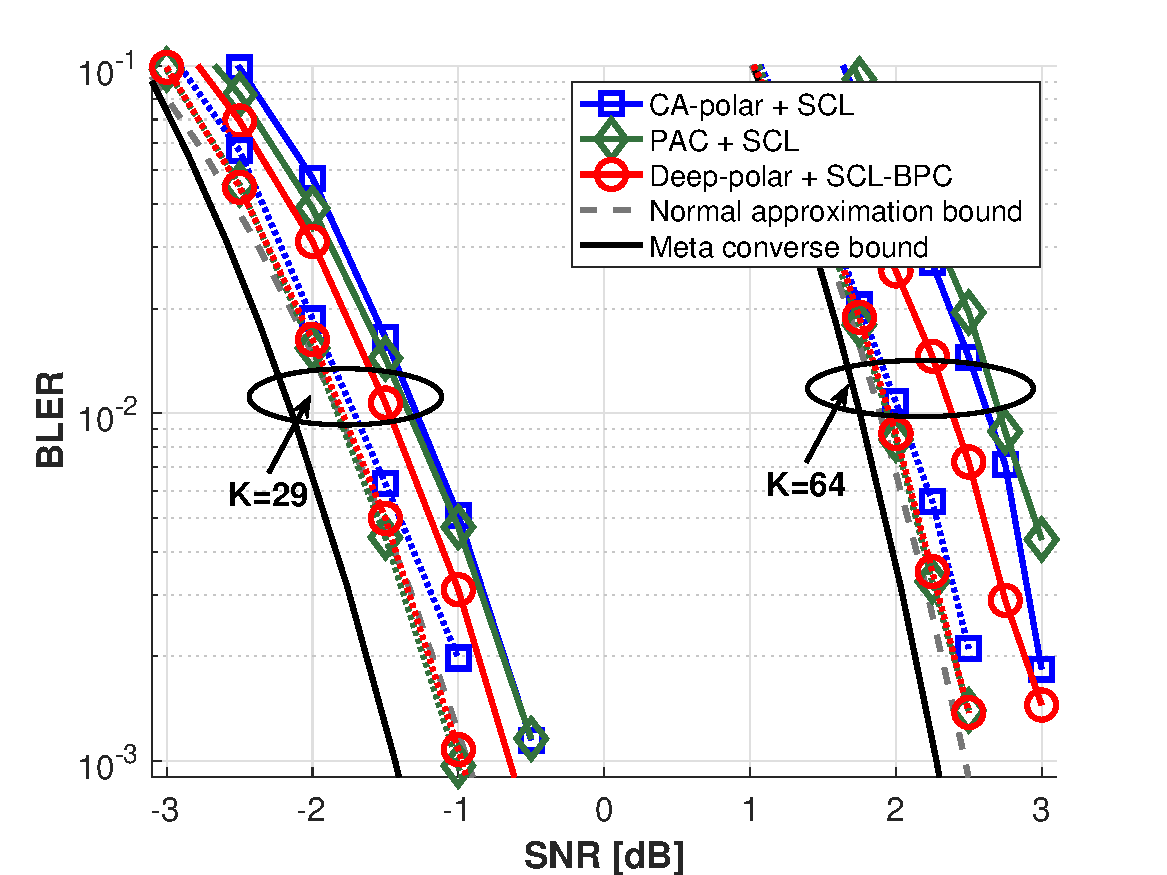
\includegraphics[width=1.1\columnwidth]{BLER_PAC_3.pdf}
\caption{BLER performance of PAC, CA-polar, and deep polar codes. Parameters for solid line are $(K,S) \in \{(29,8), (64,8)\}$, and for dotted line are $(K,S)\in \{(29,32), (64,256)\}$.}
\label{fig:BLER-PAC}
\end{figure}


\begin{figure}[t]
\centering
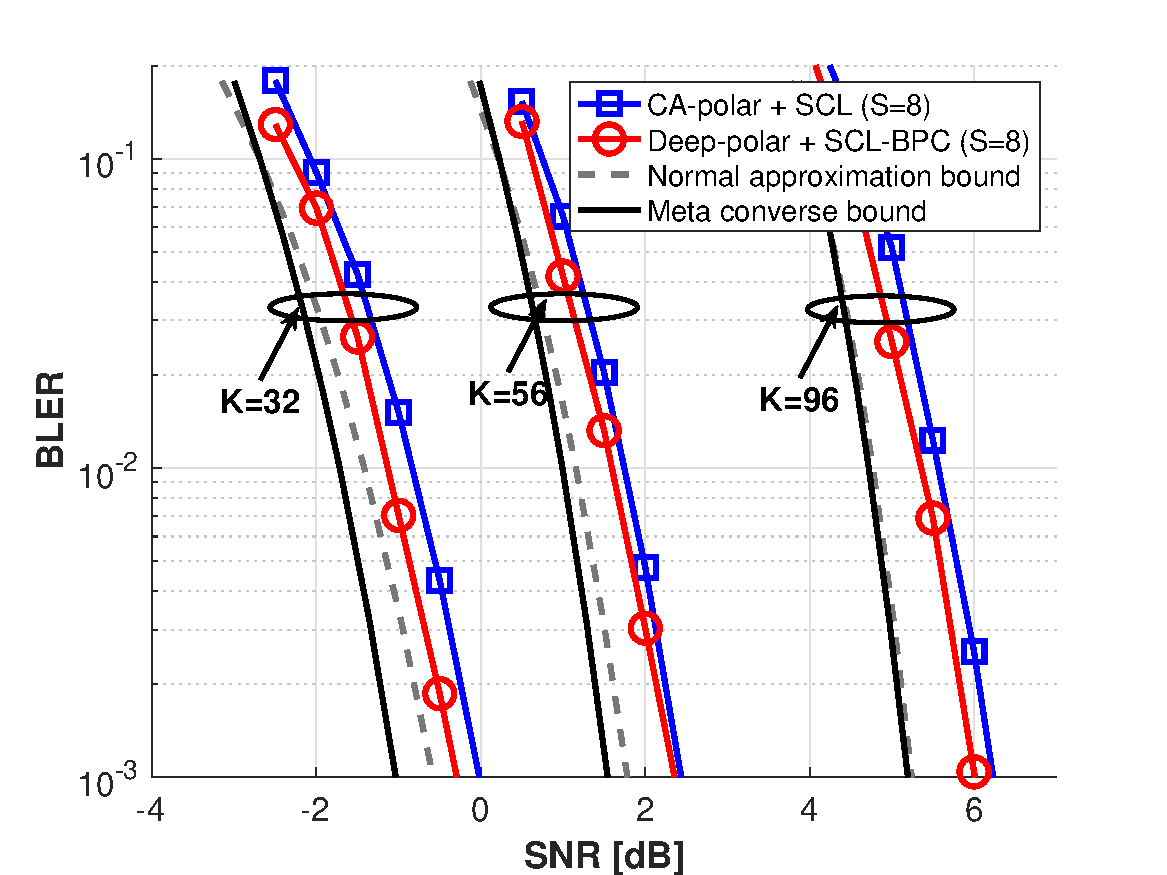
\includegraphics[width=1.1\columnwidth]{BLER_CA_polar.pdf}
\caption{BLER performance comparison bewteen deep polar and CA-polar codes. The code parameters are $N=128$ and $K\in\{32, 56, 96$\}.}
\label{fig:BLER-CA-Polar}
\end{figure}
 
 


\begin{figure}[t]
\centering
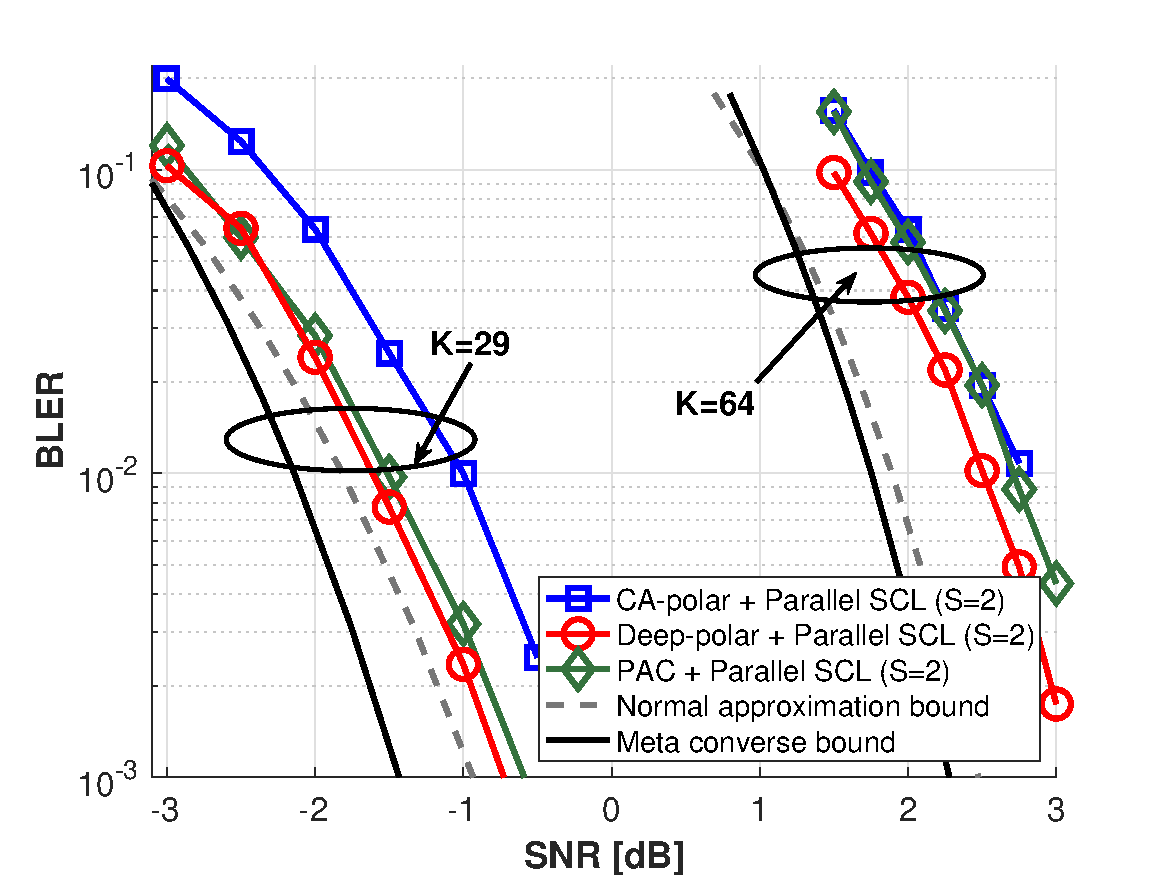
\includegraphics[width=1.1\columnwidth]{BLER_PAC_parallel.pdf}
\caption{BLER performance under parallel-SCL decoder.}
\label{fig:BLER-PAC-parallel}
\end{figure}




{\bf Comparison with CA-BOSS codes:}
Fig.~\ref{fig:BLER-BOSS} presents the ML decoding performance of four coding schemes: deep polar codes, CA-deep polar codes, CA-BOSS codes, and CA-polar codes, at different code rates $R\in \{\frac{16}{256},\frac{16}{128},\frac{16}{64}\}$. The results demonstrate the effectiveness of the proposed codes in improving the weight spectrum. By utilizing ML decoding, we assess the performance improvement achieved by the proposed codes. For example, when $R=\frac{16}{128}$, the CA-BOSS code marginally outperforms the deep polar code. However, with the integration of CRC precoding, the CA-deep polar code exhibits superior decoding performance compared to all other considered coding schemes, even achieving the meta converse bound within 0.4 dB. This remarkable outcome highlights the significant benefits of harmonizing local pre-transform (e.g., deep polar code) with global pre-transform (e.g., CRC) for boosting decoding performance at low rates. 


% The local pre-transform plays a crucial role in assisting the SCL decoder through pruning decoding paths based on the BPC principle. On the other hand, the global CRC pre-transform enhances the minimum distance of codes, facilitating the final codeword selection. The combination of these pre-transformations optimally leverages the strengths of each coding scheme, leading to substantial decoding performance improvements. Overall, these findings demonstrate the effectiveness of the proposed codes and underline the importance of intelligently integrating different pre-transformations to achieve enhanced decoding performance, particularly at low code rates.


\begin{figure}[t]
\centering
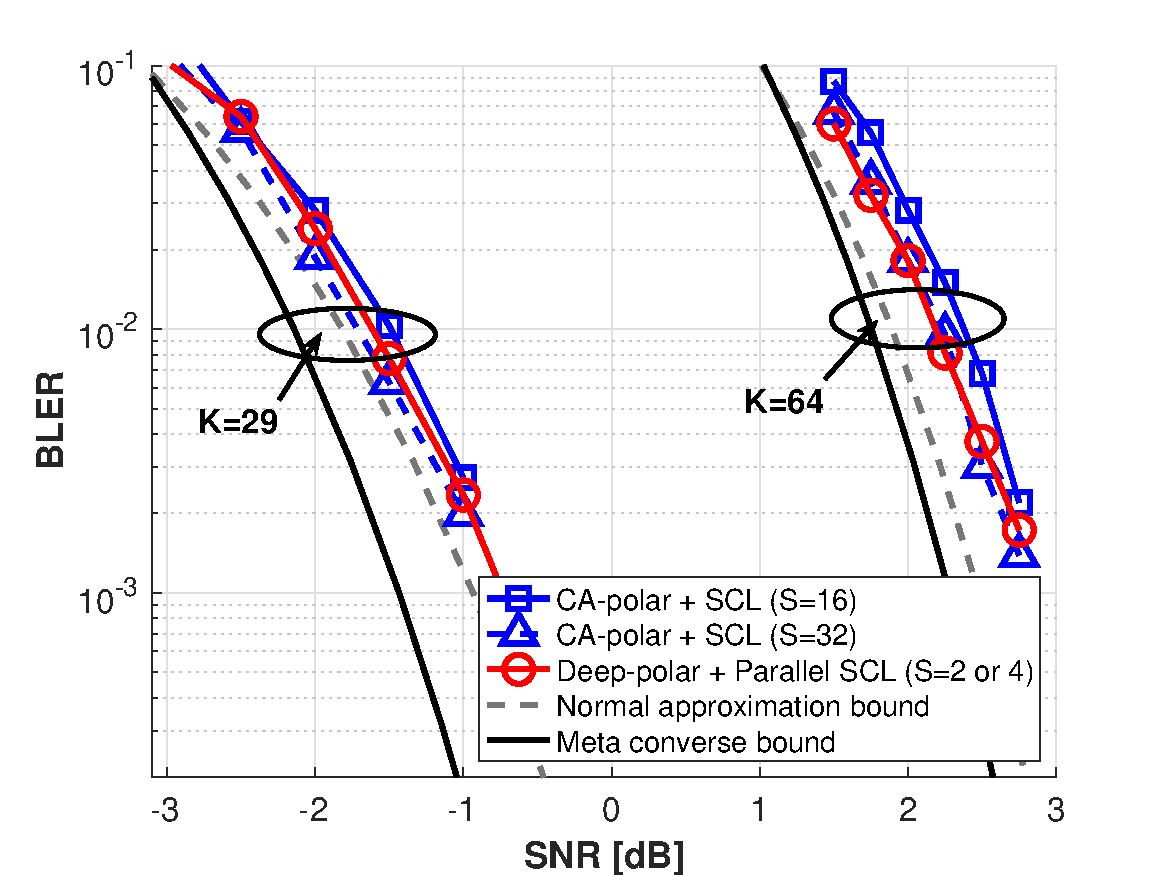
\includegraphics[width=1.1\columnwidth]{BLER_DP_parallel_2.pdf}
\caption{BLER performance of deep polar codes under parallel-SCL decoder and CA-polar codes under SCL decoder. We use list size $S=2$ for decoding deep polar codes for $K=29$, and $S=4$ for $K=64$.}
\label{fig:BLER-DP-vs-SCL}
\end{figure}



\begin{figure}[t]
\centering
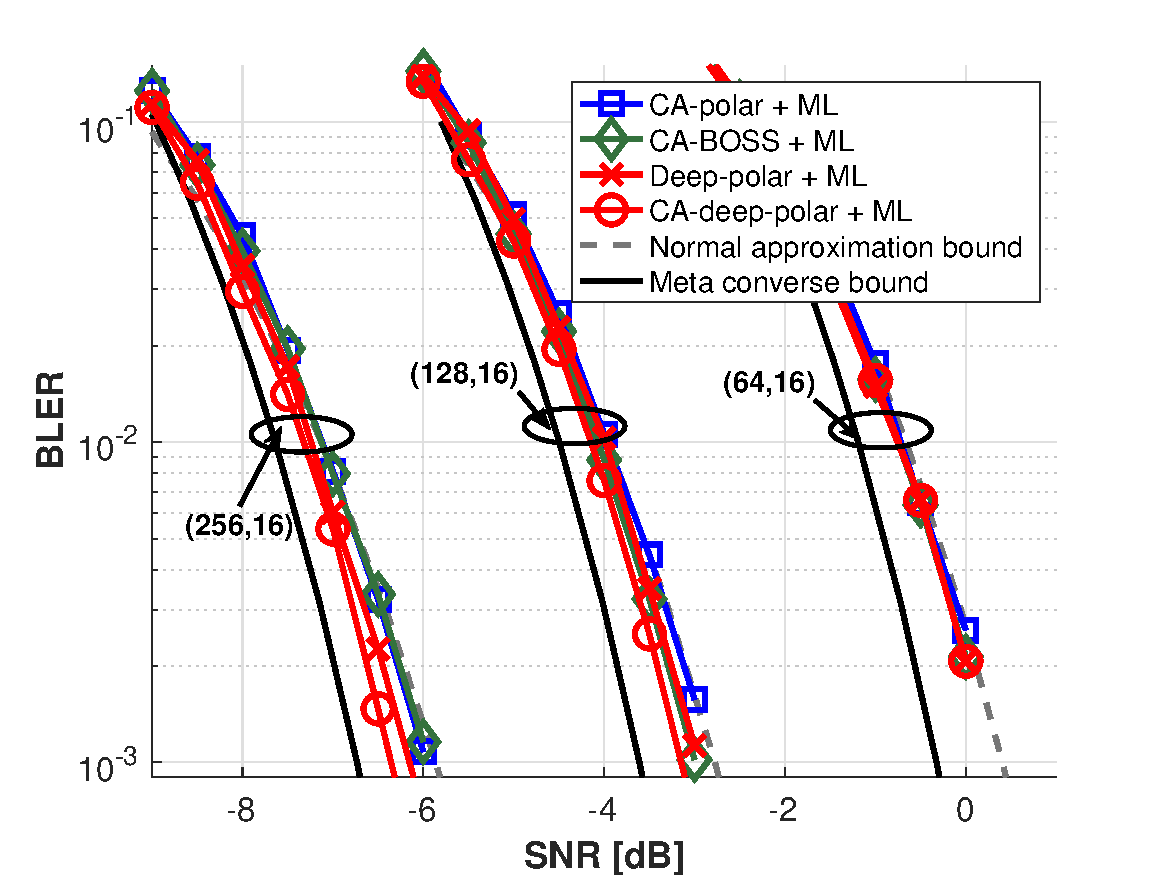
\includegraphics[width=1.1\columnwidth]{BLER_BOSS.pdf}
\caption{BLER performance of deep polar, CA-deep polar, CA-polar, and CA-BOSS codes. The CRC polynomial is $1 + D^5 + D^6$ for CA-deep polar and CA-polar codes and $1 + D + D^3$ for CA-BOSS codes.}
\label{fig:BLER-BOSS}
\end{figure}




\section{Conclusion}
 We have introduced a novel type of pre-transformed polar code called the deep polar code. The deep polar codes are generated through successive multi-layered encoding with a flexible rate-profiling method. The main technical innovation involves creating a unique yet universal pre-transformed architectures of polar codes, which is inspired by deep layered transform coding. These innovative architectures open up new possibilities for exploring a far more diverse range of pre-transformed polar code structures that were not explored before. Our deep polar code is a superposition code of pre-transformed and regular polar subcodes. Controlling the rates of these two subcodes enables the design of low-complexity decoding while significantly improving the weight distribution of the codes. Leveraging this superposition property, we have also introduced two decoding methods: the SCL-BPC decoder, which effectively reduces decoding complexity, and the parallel-SCL decoder, which minimizes decoding latency. Through simulations, we have demonstrated that our codes achieve close to finite-blocklength capacity and consistently outperform all existing state-of-the-art pre-transformed polar codes at various rates and short blocklengths, all while maintaining a reasonable decoding complexity.

A promising further research direction would be to extend the deep polar code design to moderate blocklengths, such as up to 2048, in order to bridge the gap towards the finite-blocklength capacity in moderate blocklength regimes. Additionally, exploring the development of a more efficient decoding algorithm for larger code blocklengths holds great promise, as the complexity of the SCL-BPC decoder may become computationally prohibitive in moderate blocklengths. Lastly, it is also interesting to design an efficient rate-compatible deep polar code to optimally support HARQ protocols. 


\bibliographystyle{IEEEtran}
\bibliography{Coding}

 
\end{document}
